%% ============================================================================
%% Apunte_v2.tex -- documento maestro del apunte de Ecuaciones Diferenciales.
%% Version 2 (octubre 2026). Reemplaza a "Apunte .tex".
%%
%% Que cambia respecto de la version anterior
%%   - Interruptores por capitulo (\capOrdenUnotrue, etc.) en lugar de comentar
%%     y descomentar bloques. La numeracion es fija: capitulos 1, 2 y 3, aunque
%%     los anteriores esten apagados.
%%   - Capitulo "Sistemas lineales" completo: sistemas_1_v2 + sistemas_defectuosos
%%     + practica_sistemas_1 dentro de una misma \section. Antes, los \subsection
%%     de sistemas_defectuosos quedaban sin \section (numeracion "x.0.y") y sus
%%     \ref a sistemas_1_v2 salian como "??".
%%   - Correccion de \ref en cajas numeradas movida al preambulo (vale para todos
%%     los capitulos, no solo desde sistemas_defectuosos).
%%   - Portada con la paleta de la clase (colores bbe*) en vez de azules propios;
%%     logo con ruta flexible; version y semestre como datos en un solo lugar.
%%   - Guia de lectura con la leyenda de cajas y de niveles de ejercicio.
%%   - Indice en numeracion romana (\frontmatter); paginas arabigas desde el
%%     capitulo 1 (\mainmatter).
%% ============================================================================

%% Clase: se usa la primera que exista en el proyecto (bb2_v2, bbe2 o bb2).
\IfFileExists{bb2_v2.cls}%
  {\documentclass[12pt,a4paper,blue]{bb2_v2}}%
  {\IfFileExists{bbe2.cls}%
    {\documentclass[12pt,a4paper,blue]{bbe2}}%
    {\documentclass[12pt,a4paper,blue]{bb2}}}

%% Si se carga una clase anterior a bb2_v2, este color no existe: se define aqui.
\providecolor{bbeamberdark}{HTML}{8D6115}

%% Solo "spanish": la opcion es-nodecimaldot no existe en versiones antiguas de
%% babel y detiene la compilacion. \decimalpoint (si existe) deja el punto decimal.
\usepackage[spanish]{babel}
\ifdefined\decimalpoint\decimalpoint\fi
\usepackage{amsmath,amssymb}
\usepackage{array}
\usepackage{mathrsfs}
\usepackage[many]{tcolorbox}
\usepackage{graphicx}

% --- Graficos con TikZ y PGFPlots ---
\usepackage{tikz}
\usepackage{pgfplots}
\pgfplotsset{compat=1.18}

% --- Librerias de TikZ (la clase ya carga la mayoria; repetirlas no molesta) ---
\usetikzlibrary{
    patterns,                  % patron de la pared (north east lines)
    decorations.pathmorphing,  % resorte: decoration={coil,...}
    decorations.markings,      % marcas en las flechas de los retratos de fase
    arrows.meta,               % flechas modernas
    positioning,               % nodos relativos
    calc                       % calculos de coordenadas
}

% --- Subfiguras (retratos de fase de sistemas_defectuosos) ---
\usepackage{subcaption}

%% ----------------------------------------------------------------------------
%% Datos del apunte: se cambian aqui y se actualizan portada, PDF y pie de pagina
%% ----------------------------------------------------------------------------
\newcommand{\apunteautor}{Jose David Torres-Riffo}
\newcommand{\apuntesemestre}{2026-II}
\newcommand{\apunteversion}{Versi\'on 2 \textbullet\ octubre de 2026}
\providecommand{\cursoactual}{}
\renewcommand{\cursoactual}{Apuntes EDO \textbullet\ \apuntesemestre}

\hypersetup{
  pdftitle={Apuntes de Ecuaciones Diferenciales},
  pdfauthor={\apunteautor},
  pdfsubject={Ecuaciones diferenciales y problemas aplicados}
}

%% ----------------------------------------------------------------------------
%% Colores: la portada usa los de la clase, para que coincida con capitulos y cajas
%% ----------------------------------------------------------------------------
\colorlet{primary}{bbe}
\colorlet{softblue}{bbe!8!white}

\newcommand{\deri}{\dfrac{dy}{dx}}

%% Niveles de ejercicio (identico a practica_sistemas_1.tex; \providecommand
%% evita el choque con la definicion de ese archivo).
\providecommand{\est}[1]{\textcolor{bbeamberdark}{\ifcase#1\or\ding{72}\or\ding{72}\ding{72}\or\ding{72}\ding{72}\ding{72}\fi}}

%% --- Correccion de \ref a cajas numeradas ----------------------------------
%% Con 'auto counter' de tcolorbox, \label dentro de Ejemplo/Teorema/Definicion
%% devuelve el numero de la subseccion en vez del de la caja. Este bloque fija
%% \@currentlabel dentro de cada caja. sistemas_defectuosos.tex trae el mismo
%% bloque con la misma guarda, asi que no se duplica (aqui prevalece esta
%% version). Las cajas definidas con \newtcolorbox sin contador dejan
%% \thetcbcounter vacio; una caja anonima (\begin{tcolorbox}, como la de la
%% portada) lo deja sin definir, por eso se comprueba \ifdefined primero.
\makeatletter
\ifdefined\bbereffixdone\else
  \def\bbereffixdone{}
  \tcbset{before upper={%
    \ifdefined\thetcbcounter
      \ifx\thetcbcounter\@empty\else
        \protected@edef\@currentlabel{\thetcbcounter}%
        \ifdefined\phantomsection\phantomsection\fi
      \fi
    \fi}}
\fi
\makeatother

%% Paginas en blanco (las que inserta \cleardoublepage antes de cada capitulo):
%% sin pie de pagina ni numero, como en un libro impreso.
\makeatletter
\def\cleardoublepage{\clearpage
  \if@twoside\ifodd\c@page\else
    \hbox{}\thispagestyle{empty}\newpage
    \if@twocolumn\hbox{}\thispagestyle{empty}\newpage\fi
  \fi\fi}
\makeatother

%% ----------------------------------------------------------------------------
%% Leyenda de cajas: una pastilla del color de la caja con su nombre
%% ----------------------------------------------------------------------------
\newcommand{\pastilla}[2]{%
  \tikz[baseline=(pastilla.base)]\node[draw=#1,fill=#1!10!white,text=#1!70!black,%
    inner xsep=5pt,inner ysep=2.5pt,line width=.8pt,font=\sffamily\bfseries\small](pastilla){#2};}

%% ----------------------------------------------------------------------------
%% Interruptores de capitulos: true = incluir, false = omitir
%% ----------------------------------------------------------------------------
\newif\ifcapOrdenUno      \capOrdenUnofalse      % requiere los .tex de primer orden
\newif\ifcapOrdenDos      \capOrdenDosfalse      % requiere la carpeta Capitulo_2/
\newif\ifcapSistemas      \capSistemastrue
\newif\ifincluirpractica  \incluirpracticatrue   % practica y respuestas de sistemas

\setcounter{tocdepth}{2}

%% Logo: se busca junto al documento y, si no esta, en Capitulo_2/
\newcommand{\logoapunte}[1]{%
  \IfFileExists{logo_edo.png}%
    {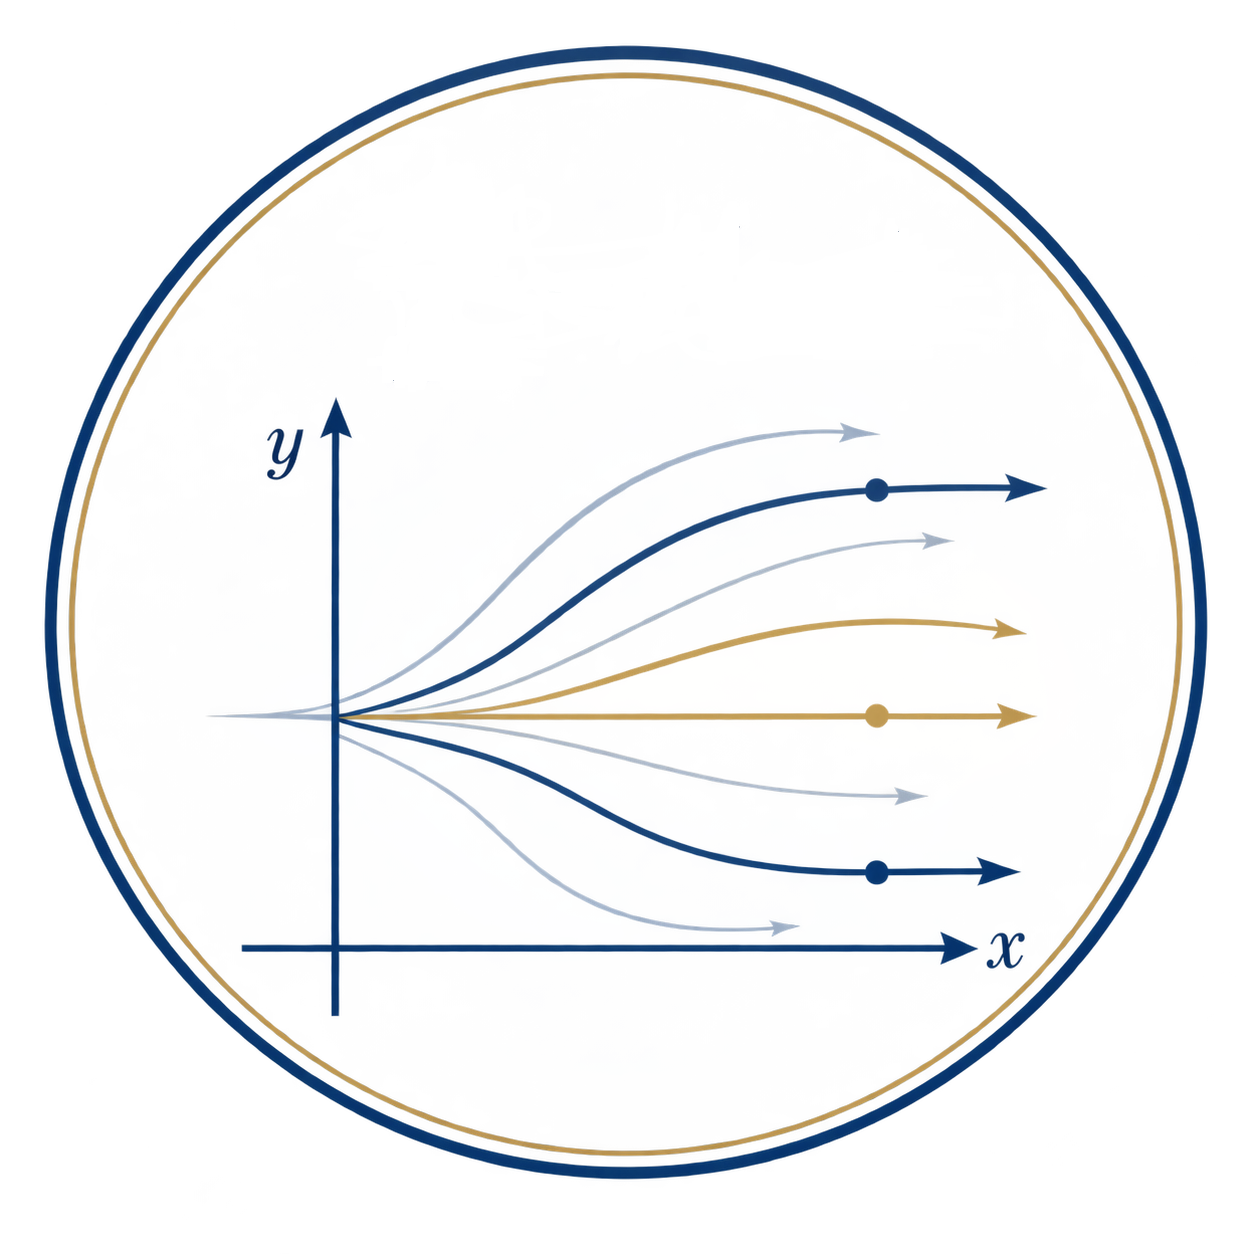
\includegraphics[width=#1]{logo_edo.png}}%
    {\IfFileExists{Capitulo_2/logo_edo.png}%
      {\includegraphics[width=#1]{Capitulo_2/logo_edo.png}}%
      {}}}

%% \entrada{archivo}: incluye el archivo desde Capitulo_3/ o, si no esta ahi,
%% desde la carpeta principal. Si no existe, avisa en el PDF en vez de detener
%% la compilacion. Usar minusculas/mayusculas EXACTAS (TeXPage distingue).
\newcommand{\entrada}[1]{%
  \IfFileExists{Capitulo_3/#1}{\input{Capitulo_3/#1}}%
  {\IfFileExists{#1}{\input{#1}}%
    {\PackageWarning{apunte}{No se encuentra #1.tex}%
     \par\noindent\textbf{[Falta el archivo #1.tex]}\par}}}

\begin{document}

\frontmatter
%% En el preliminar los capitulos sin numero (guia e indice) siguen sin forzar
%% pagina derecha: portada | guia, indice | ..., sin paginas en blanco de por medio.
\makeatletter\@openrightfalse\makeatother

% ==================================================
% PORTADA
% ==================================================
\begin{titlepage}
\centering
\sffamily

\vspace*{0.3cm}

% --- Linea superior decorativa ---
{\color{primary}\rule{0.6\textwidth}{2pt}}\par
\vspace{0.3cm}
{\color{primary!60}\rule{0.4\textwidth}{1pt}}\par

\vspace{1.2cm}

{\color{primary}\fontsize{30}{36}\selectfont\bfseries Apuntes de\par Ecuaciones Diferenciales\par}

\vspace{0.4cm}

{\color{primary!80}\Large Ecuaciones diferenciales y problemas aplicados\par}

\vspace{1cm}

{\color{primary}\rule{0.7\textwidth}{1.2pt}}\par

\vspace{0.8cm}

\logoapunte{0.45\textwidth}\par

\vspace{1cm}

% --- Cuadro de informacion ---
\begin{tcolorbox}[
    enhanced,
    rounded corners,
    arc=8pt,
    no shadow,
    colback=softblue!70,
    colframe=primary!40,
    boxrule=1pt,
    width=0.7\textwidth,
    halign=center,
    before skip=0pt,
    after skip=0pt
]
{\color{primary}\large\bfseries \apunteautor}
\end{tcolorbox}

\vspace{0.4cm}

{\color{primary}\large \apuntesemestre\par}
\vspace{0.1cm}
{\color{primary!70}\small \apunteversion\par}

\vfill

% --- Linea inferior decorativa ---
{\color{primary!60}\rule{0.4\textwidth}{1pt}}\par
\vspace{0.3cm}
{\color{primary}\rule{0.6\textwidth}{2pt}}\par

\end{titlepage}

% ==================================================
% GUIA DE LECTURA
% ==================================================
\chapter*{C\'omo usar este apunte}

Este apunte est\'a pensado para trabajarse con l\'apiz en mano. Los temas se desarrollan con ejemplos resueltos paso a paso y se acompa\~nan de secciones de problemas. Antes de leer la soluci\'on de un ejemplo, intenta resolverlo por tu cuenta; despu\'es compara tu camino con el del texto.

\subsubsection*{Las cajas}

Cada tipo de caja tiene un color y un nombre. El nombre siempre est\'a escrito, de modo que el apunte se entiende igual en una impresi\'on en blanco y negro.

\begin{center}
\renewcommand{\arraystretch}{1.9}
\begin{tabular}{@{}r p{.64\linewidth}@{}}
\pastilla{bbeblue}{Definici\'on} & Fija el significado de un t\'ermino o de una notaci\'on. \\
\pastilla{bbeblue}{Teorema}      & Resultado que se usa para resolver; su enunciado va en cursiva. \\
\pastilla{bbegreen}{Ejemplo}     & Problema resuelto paso a paso. \\
\pastilla{bbered}{Ejercicio}     & Problema para que lo resuelvas t\'u. \\
\pastilla{bbeamber}{Observaci\'on} & Comentario que conecta ideas o advierte un detalle. \\
\pastilla{bbeamber}{Obs.}        & Nota breve: una verificaci\'on o una elecci\'on alternativa. \\
\end{tabular}
\end{center}

\subsubsection*{Los niveles de los ejercicios}

Cada ejercicio de las secciones de pr\'actica indica su dificultad con estrellas. Cuando una pr\'actica trae respuestas, est\'an al final de la misma secci\'on: intenta cada ejercicio antes de consultarlas.

\begin{center}
\renewcommand{\arraystretch}{1.5}
\begin{tabular}{@{}l l p{.55\linewidth}@{}}
\est{1} & \textbf{Directo}     & Aplicaci\'on inmediata de una definici\'on, un teorema o un procedimiento visto. \\
\est{2} & \textbf{Intermedio}  & Combina varios pasos o exige elegir el m\'etodo y justificar. \\
\est{3} & \textbf{Avanzado}    & Demostraciones, casos con estructura especial o problemas de modelaci\'on. \\
\end{tabular}
\end{center}

\tableofcontents

%% Desde aqui, cada capitulo vuelve a abrir en pagina derecha.
\makeatletter\@openrighttrue\makeatother
\mainmatter

% ==================================================
% CAPITULO 1 -- Ecuaciones de primer orden
% ==================================================
%\ifcapOrdenUno
%\setcounter{chapter}{0}
%\chapter{Ecuaciones de primer orden}

%\section{El origen de las ecuaciones diferenciales}
%\begin{definition}
%    Primeros acercamientos
%\end{definition}

%\section{Terminolog\'ia e ideas b\'asicas}
%\input{basicos}

%\section{Ecuaciones separables}
%\input{separable}
%\newpage

%\section{Ecuaciones lineales de primer orden}
%\input{lineales}
%\newpage

%\section{Cambio de variables}
%\input{cambio_variables}
%\newpage

%\section{Ecuaciones Exactas}
%\input{exactas}
%\newpage

%\section{Aplicaciones}
%\input{aplicaciones}
%\newpage

%\section{Otros acercamientos, cualitativos}
%\input{cualitativo}
%\newpage

%\section{Otros acercamientos, num\'ericos}
%\input{numerico}
%\newpage

%\section{Problemas}
%\input{EDO 2025/evaluaciones/ejercicios}
%\newpage

%\section{Problemas 2}
%\input{EDO 2025/Ejercicios_2}
%\fi

% ==================================================
% CAPITULO 2 -- Ecuaciones de segundo orden
% ==================================================
\ifcapOrdenDos
\setcounter{chapter}{1}
\chapter{Ecuaciones de segundo orden}

\section{Ecuaciones homog\'eneas}
El primer tipo de ecuaci\'on de segundo orden que revisaremos ser\'a la ecuaci\'on homog\'enea de coeficientes constantes, la cual es:
\[
ay''+by'+cy=0,
\]
donde $a,b,c\in\mathbb{R}$ y $a\neq 0$. Este tipo de ecuaciones emerge de manera natural en problemas del tipo masa-resorte. La ecuaci\'on se dice homog\'enea, ya que no hay una funci\'on externa (fuerza) $f(t)$. En el caso en que existe una fuerza externa, la ecuaci\'on de coeficientes constantes se convierte en:
\[
ay''+by'+cy=f(t).
\]

La idea para resolver la ecuaci\'on homog\'enea se la debemos nuevamente al gran L.~Euler y se trata de lo siguiente: buscamos una funci\'on $y$ para la cual su segunda derivada sea una combinaci\'on de la funci\'on buscada y de su primera derivada. Esta simple idea sugiere pensar en funciones del tipo $y=e^{rt}$, ya que sus derivadas son m\'ultiplos de ella misma. De hecho, si reemplazamos:
\[
ar^2e^{rt}+bre^{rt}+ce^{rt}=0\Longrightarrow e^{rt}(ar^2+br+c)=0.
\]
Como la funci\'on $e^{rt}$ nunca es cero, tenemos que
\[
ar^2+br+c=0.
\]
A esta ecuaci\'on la llamaremos la \textbf{ecuaci\'on auxiliar} (o caracter\'istica) de la ecuaci\'on homog\'enea de coeficientes constantes.

\begin{example}
  Consideremos la ecuaci\'on dada por:
  \[
  y''+5y'-6y=0.
  \]
  Su respectiva ecuaci\'on auxiliar es:
  \[
  r^2+5r-6=(r-1)(r+6)=0,
  \]
  por lo tanto, las funciones $e^{t}$ y $e^{-6t}$ son soluciones de la ecuaci\'on dada.
\end{example}
\newpage
%[Principio de superposici\'on]
\begin{remark}
    Notemos que la funci\'on $y(t)\equiv 0$ siempre es soluci\'on de la ecuaci\'on homog\'enea. M\'as a\'un, dadas dos soluciones $y_1,y_2$ de ella y dos constantes $c_1,c_2\in \mathbb{R}$, la funci\'on
    \[
    y(t)=c_1y_1(t)+c_2y_2(t)
    \]
    es tambi\'en soluci\'on. Esto es f\'acil de verificar reemplazando en la ecuaci\'on homog\'enea y usando la linealidad de la derivada:
    \begin{align*}
      &a(c_1y_1+c_2y_2)''+b(c_1y_1+c_2y_2)'+c(c_1y_1+c_2y_2)\\
      &\qquad= a(c_1y_1''+c_2y_2'')+b(c_1y_1'+c_2y_2')+c(c_1y_1+c_2y_2)\\
      &\qquad= c_1\underbrace{(ay_1''+by_1'+cy_1)}_{=0}+c_2\underbrace{(ay_2''+by_2'+cy_2)}_{=0}=0.
    \end{align*}
    Los dos grados de libertad que entregan las constantes $c_1,c_2$ nos sugieren que, a diferencia de las ecuaciones de orden uno, las ecuaciones de segundo orden requieren m\'as condiciones iniciales para poder determinar soluciones particulares.

    En t\'erminos de un sistema mec\'anico, no nos basta con la posici\'on inicial $y(0)$: tambi\'en requerimos la velocidad inicial del sistema $y'(0)$ para determinar su comportamiento. A modo de ejemplo, un PVI de segundo orden se ve como a continuaci\'on.
\end{remark}

\begin{example}
     Considere el PVI dado por
     \[
     y''+2y'-y=0,\qquad y(0)=0,\qquad y'(0)=-1.
     \]
     Al igual que en el ejemplo anterior, utilizamos la ecuaci\'on auxiliar para encontrar las soluciones de la forma $y(t)=e^{rt}$. En este caso,
     \[
     r^2+2r-1=0\Longrightarrow r_1=-1+\sqrt{2},\qquad r_2=-1-\sqrt{2}.
     \]
     Con lo cual la soluci\'on general ser\'a:
     \[
     y(t)=c_1e^{(-1+\sqrt{2})t}+c_2e^{(-1-\sqrt{2})t}.
     \]
     A continuaci\'on debemos determinar los valores de $c_1,c_2$ a partir de los valores iniciales dados, es decir:
     \begin{align*}
         y(0)&=c_1e^0+c_2e^0,\\
         y'(0)&=(-1+\sqrt{2})c_1e^0+(-1-\sqrt{2})c_2e^0,
     \end{align*}
     de lo anterior tenemos el sistema de ecuaciones:
     \begin{align*}
         0&=c_1+c_2,\\
         -1&=(-1+\sqrt{2})c_1+(-1-\sqrt{2})c_2.
     \end{align*}
     De la primera ecuaci\'on, $c_2=-c_1$; reemplazando en la segunda obtenemos $2\sqrt{2}\,c_1=-1$. Por lo tanto $c_1=-\dfrac{\sqrt{2}}{4}$, $c_2=\dfrac{\sqrt{2}}{4}$, y la respectiva soluci\'on particular es:
     \[
     y(t)=-\dfrac{\sqrt{2}}{4}e^{(-1+\sqrt{2})t}+\dfrac{\sqrt{2}}{4}e^{(-1-\sqrt{2})t}.
     \]
\end{example}

En el cap\'itulo anterior revisamos un teorema que nos aseguraba, bajo ciertas condiciones, la existencia y unicidad de soluci\'on para las ecuaciones de orden uno. A continuaci\'on revisaremos el resultado equivalente para PVI con ecuaciones de orden dos.

\begin{theorem}[Existencia y unicidad]
    Para cualquier colecci\'on de n\'umeros reales $a,b,c,t_0,Y_0,Y_1$ con $a\neq 0$, existe una \'unica soluci\'on del problema de valor inicial
    \[
    ay''+by'+cy=0,\qquad y(t_0)=Y_0,\qquad y'(t_0)=Y_1,
    \]
    y esta soluci\'on es v\'alida para todo $t\in\, ]-\infty,\infty[$.
\end{theorem}

Como veremos a continuaci\'on, el hecho de que el teorema anterior nos asegure la unicidad de la soluci\'on es de gran ayuda: nos bastar\'a encontrar (de cualquier manera) dos soluciones $y_1,y_2$ que sean \emph{esencialmente distintas} para que la funci\'on $c_1y_1+c_2y_2$, con constantes adecuadas, sea la soluci\'on buscada. Notemos que no basta con que sean distintas: por ejemplo, $e^{t}$ y $2e^{t}$ son distintas, pero cualquier combinaci\'on de ellas es de la forma $Ce^{t}$, y con una sola constante no podemos satisfacer dos condiciones iniciales. Para precisar esta idea, definimos el siguiente concepto.

\begin{definition}
    Dos funciones $y_1(t),\,y_2(t)$ se dicen \textbf{linealmente independientes} (L.I.) sobre el intervalo $I\subseteq \mathbb{R}$ si la \'unica forma de tener
    \[
    c_1y_1(t)+c_2y_2(t)=0\quad\text{para todo } t\in I
    \]
    es con $c_1=c_2=0$. En caso contrario diremos que las funciones son \textbf{linealmente dependientes} (L.D.) sobre $I$.

    Para dos funciones, esto equivale a decir que ninguna de ellas es un m\'ultiplo constante de la otra en $I$; es decir, no existe una constante $k$ tal que $y_1(t)=k\,y_2(t)$ para todo $t\in I$ (ni $y_2(t)=k\,y_1(t)$ para todo $t\in I$).
\end{definition}

\begin{example}
    Las funciones
    \[
    y_1(t)=\sin(t)\cos(t),\qquad y_2(t)=\sin(2t)
    \]
    son linealmente dependientes en $\mathbb{R}$, ya que por la identidad del \'angulo doble $y_1(t)=\tfrac{1}{2}\,y_2(t)$ para todo $t$.

    En cambio, las funciones
    \[
    y_1(t)=e^{t},\qquad y_2(t)=e^{4t}
    \]
    son linealmente independientes en $\mathbb{R}$, pues el cociente $y_2(t)/y_1(t)=e^{3t}$ no es constante.
\end{example}

Para verificar la independencia lineal de manera sistem\'atica, introducimos la siguiente herramienta.

\begin{definition}
    Dadas dos funciones derivables $y_1,y_2$, se define el \textbf{Wronskiano} de ellas como:
    \[
    W[y_1,y_2](t)=\begin{vmatrix}
        y_1(t) & y_2(t)\\
        y_1'(t) & y_2'(t)
    \end{vmatrix}=y_1(t)y_2'(t)-y_1'(t)y_2(t).
    \]
\end{definition}

\begin{remark}
    Si existe al menos un punto $t_0\in I$ tal que $W[y_1,y_2](t_0)\neq 0$, entonces las funciones $y_1,y_2$ son L.I. en $I$.

    El rec\'iproco es falso para funciones arbitrarias: por ejemplo, $y_1(t)=t^2$ e $y_2(t)=t|t|$ tienen Wronskiano id\'enticamente nulo en $\mathbb{R}$ y, sin embargo, son L.I. en $\mathbb{R}$. No obstante, cuando $y_1,y_2$ son \emph{soluciones} de la ecuaci\'on homog\'enea, su Wronskiano o bien es id\'enticamente cero, o bien no se anula nunca (esto lo justificaremos m\'as adelante con la f\'ormula de Abel). En ese caso, las soluciones son L.I. si y solo si su Wronskiano es distinto de cero.
\end{remark}

\begin{example}
    Para las funciones $y_1(t)=e^{t}$, $y_2(t)=e^{4t}$ se tiene:
    \[
    W[y_1,y_2](t)=\begin{vmatrix}
        e^t & e^{4t}\\
        e^t & 4e^{4t}
    \end{vmatrix}=4e^{5t}-e^{5t}=3e^{5t}\neq 0,\qquad \forall\, t\in\, ]-\infty,\infty[,
    \]
    lo que confirma que son L.I.
\end{example}

El siguiente resultado relaciona la existencia de soluciones con los conceptos reci\'en introducidos.

\begin{theorem}
    Si $y_1(t),y_2(t)$ son dos soluciones L.I. en $]-\infty,\infty[$ de la ecuaci\'on de coeficientes constantes, entonces existen \'unicas constantes $c_1,c_2$ de manera que $c_1y_1(t)+c_2y_2(t)$ satisface el problema de valor inicial
    \[
    ay''+by'+cy=0,\qquad y(t_0)=Y_0,\qquad y'(t_0)=Y_1,
    \]
    en dicho intervalo. Por esta raz\'on, a la expresi\'on $y_h=c_1y_1+c_2y_2$ la llamamos \textbf{soluci\'on general} de la ecuaci\'on homog\'enea.
\end{theorem}

\begin{remark}
    Es instructivo ver d\'onde aparece el Wronskiano en el teorema anterior. Imponer las condiciones iniciales a $c_1y_1+c_2y_2$ lleva al sistema
    \begin{align*}
        c_1y_1(t_0)+c_2y_2(t_0)&=Y_0,\\
        c_1y_1'(t_0)+c_2y_2'(t_0)&=Y_1,
    \end{align*}
    cuyo determinante es exactamente $W[y_1,y_2](t_0)$. Por lo tanto, el sistema tiene soluci\'on \'unica $(c_1,c_2)$ precisamente cuando $W[y_1,y_2](t_0)\neq 0$, es decir, cuando las soluciones son L.I.
\end{remark}

Para la ecuaci\'on de coeficientes constantes tenemos, por lo tanto, tres casos seg\'un el tipo de ra\'ices de la ecuaci\'on auxiliar.

\subsection*{Caso 1: ra\'ices reales y distintas}

\begin{theorem}
    Si la ecuaci\'on auxiliar $ar^2+br+c=0$ posee dos soluciones reales y distintas $r_1,r_2$, entonces la ecuaci\'on homog\'enea tiene por soluci\'on general:
    \[
    y_h=c_1e^{r_1t}+c_2e^{r_2t}.
    \]
\end{theorem}

En efecto, $W[e^{r_1t},e^{r_2t}](t)=(r_2-r_1)e^{(r_1+r_2)t}\neq 0$, pues $r_1\neq r_2$. Este es el caso que encontramos en los dos primeros ejemplos de la secci\'on.

\subsection*{Caso 2: una ra\'iz real doble}

\begin{theorem}
    Si la ecuaci\'on auxiliar $ar^2+br+c=0$ posee una \'unica ra\'iz real $r$ (ra\'iz doble), entonces la ecuaci\'on homog\'enea tiene por soluci\'on general:
    \[
    y_h=c_1e^{rt}+c_2te^{rt}.
    \]
\end{theorem}

\begin{proof}[Justificaci\'on]
    Si $r$ es ra\'iz doble, entonces $r=-\dfrac{b}{2a}$, es decir, $2ar+b=0$. Para $y=te^{rt}$ tenemos $y'=(1+rt)e^{rt}$ e $y''=(2r+r^2t)e^{rt}$, luego
    \[
    ay''+by'+cy=e^{rt}\big[t\underbrace{(ar^2+br+c)}_{=0}+\underbrace{(2ar+b)}_{=0}\big]=0.
    \]
    Adem\'as, $W[e^{rt},te^{rt}](t)=e^{2rt}\neq 0$, por lo que ambas soluciones son L.I.
\end{proof}

\begin{example}
    Consideremos la ecuaci\'on
    \[
    y''+4y'+4y=0.
    \]
    Su ecuaci\'on auxiliar es $r^2+4r+4=(r+2)^2=0$, que tiene una \'unica ra\'iz $r=-2$. Con esto, por el resultado anterior,
    \[
    y_h(t)=c_1e^{-2t}+c_2te^{-2t}.
    \]
    Verifiquemos directamente que $y_2(t)=te^{-2t}$ es soluci\'on de nuestra ecuaci\'on:
    \begin{align*}
        y_2(t)&=te^{-2t},\\
        y_2'(t)&=e^{-2t}-2te^{-2t},\\
        y_2''(t)&=-4e^{-2t}+4te^{-2t},
    \end{align*}
    y reemplazando:
    \[
    y_2''+4y_2'+4y_2=\left(-4e^{-2t}+4te^{-2t}\right)+4\left(e^{-2t}-2te^{-2t}\right)+4te^{-2t}=0.
    \]
\end{example}

\subsection*{Caso 3: ra\'ices complejas conjugadas}

\begin{theorem}
    Si la ecuaci\'on auxiliar posee ra\'ices complejas $\alpha\pm i\beta$ (con $\beta\neq 0$), entonces dos soluciones linealmente independientes de la ecuaci\'on de coeficientes constantes son:
    \[
    y_1(t)=e^{\alpha t}\cos(\beta t),\qquad y_2(t)=e^{\alpha t}\sin(\beta t).
    \]
    Por lo tanto, la soluci\'on general es:
    \[
    y(t)=c_1e^{\alpha t}\cos(\beta t)+c_2e^{\alpha t}\sin(\beta t),
    \]
    donde $c_1,c_2$ son constantes reales.
\end{theorem}

\begin{proof}[Justificaci\'on]
    La funci\'on compleja $e^{(\alpha+i\beta)t}$ es soluci\'on de la ecuaci\'on, pues $\alpha+i\beta$ es ra\'iz de la ecuaci\'on auxiliar. Por la f\'ormula de Euler,
    \[
    e^{(\alpha+i\beta)t}=e^{\alpha t}\cos(\beta t)+i\,e^{\alpha t}\sin(\beta t).
    \]
    Como los coeficientes $a,b,c$ son reales, al reemplazar en la ecuaci\'on la parte real y la parte imaginaria deben anularse por separado; por lo tanto, $e^{\alpha t}\cos(\beta t)$ y $e^{\alpha t}\sin(\beta t)$ son soluciones reales. Su Wronskiano es $\beta e^{2\alpha t}\neq 0$, as\'i que son L.I.
\end{proof}

\begin{example}
    Determine la soluci\'on del problema de valor inicial
    \[
    y''+2y'+2y=0,\qquad y(0)=0,\qquad y'(0)=2.
    \]
    La respectiva ecuaci\'on auxiliar es $r^2+2r+2=0$, la cual tiene por soluciones
    \[
    r=-1\pm i\Longrightarrow \alpha=-1,\quad \beta=1.
    \]
    Con lo cual, la soluci\'on general es:
    \[
    y(t)=c_1e^{-t}\cos(t)+c_2e^{-t}\sin(t).
    \]
    Luego debemos calcular las respectivas constantes. De $y(0)=0$ obtenemos $c_1=0$. Derivando,
    \[
    y'(t)=e^{-t}\big[(c_2-c_1)\cos(t)-(c_1+c_2)\sin(t)\big],
    \]
    y de $y'(0)=c_2-c_1=2$ obtenemos $c_2=2$. Por lo tanto, la soluci\'on del PVI es
    \[
    y(t)=2e^{-t}\sin(t).
    \]
\end{example}

\subsection*{Resumen}

\begin{center}
\renewcommand{\arraystretch}{1.4}
\begin{tabular}{|c|c|}
\hline
\textbf{Ra\'ices de } $ar^2+br+c=0$ & \textbf{Soluci\'on general} \\ \hline
$r_1\neq r_2$ reales & $c_1e^{r_1t}+c_2e^{r_2t}$ \\ \hline
$r_1=r_2=r$ real & $c_1e^{rt}+c_2te^{rt}$ \\ \hline
$\alpha\pm i\beta$ complejas & $e^{\alpha t}\big(c_1\cos(\beta t)+c_2\sin(\beta t)\big)$ \\ \hline
\end{tabular}
\end{center}

Estos casos se pueden extender f\'acilmente a ecuaciones de orden mayor que dos. Si bien no es el objetivo de este cap\'itulo, mostraremos un ejemplo para fijar la idea general.

\begin{example}
    Consideremos la ecuaci\'on:
    \[
    y'''+3y''-y'-3y=0,
    \]
    la cual tiene asociada la ecuaci\'on auxiliar $r^3+3r^2-r-3=0$. Agrupando t\'erminos, esta ecuaci\'on se puede factorizar como
    \[
    r^3+3r^2-r-3=r^2(r+3)-(r+3)=(r-1)(r+1)(r+3)=0,
    \]
    con lo cual la respectiva soluci\'on general es:
    \[
    y_h=c_1e^{t}+c_2e^{-t}+c_3e^{-3t}.
    \]
\end{example}

\newpage
\subsection*{Aplicaci\'on: el sistema masa-resorte}

\begin{remark}
    Como mencionamos anteriormente, la mec\'anica del modelo masa-resorte se rige por la segunda ley de Newton: la posici\'on de un objeto de masa $m$ en el tiempo $t$ est\'a dada por $y(t)$, que satisface la ecuaci\'on
    \[
    my''(t)+by'(t)+ky(t)=0,
    \]
    cuyos t\'erminos se pueden identificar f\'isicamente como
    \[
    \text{[inercia]}\,y''+\text{[amortiguaci\'on]}\,y'+\text{[rigidez]}\,y=0.
    \]
    En un sistema f\'isico usual se tiene $m>0$, $b\geq 0$ y $k>0$.
\end{remark}

\begin{example}
    Determine la ecuaci\'on de movimiento para el sistema masa-resorte con
    $m=36\,\mathrm{kg}$, $b=12\,\mathrm{kg/s}$ y $k=37\,\mathrm{kg/s^2}$, donde las condiciones iniciales son $y(0)=0{,}7\,\mathrm{m}$ e $y'(0)=0{,}1\,\mathrm{m/s}$.

    La ecuaci\'on es $36y''+12y'+37y=0$, con ecuaci\'on auxiliar $36r^2+12r+37=0$. Su discriminante es $144-4\cdot 36\cdot 37=-5184=-72^2$, luego
    \[
    r=\frac{-12\pm 72i}{72}=-\frac{1}{6}\pm i\Longrightarrow \alpha=-\frac{1}{6},\quad \beta=1,
    \]
    y la soluci\'on general es
    \[
    y(t)=c_1e^{-t/6}\cos(t)+c_2e^{-t/6}\sin(t).
    \]
    De $y(0)=0{,}7$ obtenemos $c_1=0{,}7$. Adem\'as,
    \[
    y'(0)=-\frac{c_1}{6}+c_2=0{,}1\Longrightarrow c_2=0{,}1+\frac{0{,}7}{6}=\frac{13}{60}.
    \]
    Por lo tanto, la ecuaci\'on de movimiento es
    \[
    y(t)=0{,}7\,e^{-t/6}\cos(t)+\frac{13}{60}\,e^{-t/6}\sin(t).
    \]
    El factor $e^{-t/6}$ hace que la amplitud de las oscilaciones decaiga con el tiempo: es un movimiento \textbf{subamortiguado}.

    \begin{center}
        \includegraphics[width=0.8\textwidth]{Capitulo_2/grafico_resorte_v2.png}
    \end{center}
\end{example}

\begin{example}
    Considere ahora la ecuaci\'on
    \[
    36y''-12y'+37y=0.
    \]
    Su ecuaci\'on auxiliar tiene ra\'ices $r=\frac{1}{6}\pm i$, por lo que su soluci\'on general es:
    \[
    y(t)=c_1e^{t/6}\cos(t)+c_2e^{t/6}\sin(t).
    \]
    Observe que el \'unico cambio respecto del ejemplo anterior es el signo del coeficiente de $y'$. Un coeficiente de amortiguaci\'on negativo no corresponde a un resorte usual (ser\'ia un sistema que \emph{inyecta} energ\'ia), y su efecto es que ahora el factor $e^{t/6}$ hace crecer la amplitud de las oscilaciones sin l\'imite, como se aprecia en el gr\'afico:
    \begin{center}
        \includegraphics[width=0.6\textwidth]{Capitulo_2/masa_resorte_2.png}
    \end{center}
\end{example}

\begin{example}
    Considere la ecuaci\'on
    \[
    y''+5y'-6y=0,
    \]
    que tiene por soluci\'on general:
    \[
    y_h=c_1e^{t}+c_2e^{-6t}.
    \]
    Si imponemos la condici\'on inicial $y(0)=1$ con una velocidad inicial $y'(0)=v_0$, obtenemos el sistema $c_1+c_2=1$, $c_1-6c_2=v_0$, cuya soluci\'on da
    \[
    y(t)=\dfrac{6+v_0}{7}e^{t}+\dfrac{1-v_0}{7}e^{-6t}.
    \]
    Observe que el t\'ermino $e^{t}$ crece sin l\'imite, mientras que $e^{-6t}$ tiende a cero. Por lo tanto, la soluci\'on tiende a cero cuando $t\to\infty$ \emph{\'unicamente} si $v_0=-6$; para cualquier otra velocidad inicial, la soluci\'on diverge a $+\infty$ (si $v_0>-6$) o a $-\infty$ (si $v_0<-6$). Esto se puede visualizar como:
    \begin{center}
        \includegraphics[width=0.7\textwidth]{Capitulo_2/masa_resorte_3.png}
    \end{center}
\end{example}

\newpage

\section{Coeficientes indeterminados}
En esta secci\'on nuestro objetivo ser\'a encontrar una soluci\'on, a la que llamaremos \textbf{soluci\'on particular}, de ecuaciones del tipo:
\[
ay''+by'+cy=f(t).
\]
Si bien de la secci\'on anterior ya sabemos que la respectiva ecuaci\'on homog\'enea posee infinitas soluciones, por el momento nos contentaremos con encontrar una soluci\'on particular. M\'as adelante veremos c\'omo combinar ambas.

Para fijar la idea de los casos que trataremos, comencemos con un ejemplo.

\begin{example}
    Determine una soluci\'on particular de:
    \[
    y''+3y'+2y=3t.
    \]
    En este caso buscamos una funci\'on $y=y(t)$ tal que una combinaci\'on lineal de ella y sus derivadas genere la funci\'on lineal $3t$. Una apuesta natural es pensar que la funci\'on que buscamos debe ser tambi\'en de tipo lineal, digamos $y(t)=At+B$, con $A,B$ constantes a determinar. De aqu\'i tenemos:
    \[
    y'(t)=A,\qquad y''(t)=0,
    \]
    y reemplazando en la ecuaci\'on dada,
    \[
    y''+3y'+2y=3t\Longrightarrow 0+3A+2(At+B)=3t\Longrightarrow 2At+(3A+2B)=3t.
    \]
    Igualando los coeficientes de $t$ y los t\'erminos constantes obtenemos $2A=3$ y $3A+2B=0$, sistema que al resolver nos entrega $A=\dfrac{3}{2}$, $B=-\dfrac{9}{4}$. Por lo tanto, la funci\'on
    \[
    y_p(t)=\dfrac{3}{2}t-\dfrac{9}{4}
    \]
    es una soluci\'on particular de la ecuaci\'on dada.
\end{example}

\begin{figure}[h!]
    \centering
    \begin{tikzpicture}
        \begin{axis}[
            axis lines = middle,
            xlabel = $t$,
            ylabel = {$y$},
            ymin=-5, ymax=10,
            xmin=-1, xmax=3.5,
            legend pos = north west,
            grid = both,
            minor tick num = 1,
            major grid style = {lightgray},
            minor grid style = {lightgray!25},
            width = 10cm,
            height = 7cm
        ]
        % Funcion forzadora f(t) = 3t
        \addplot[domain=-1:3.3, samples=100, color=blue, thick] {3*x};
        \addlegendentry{$f(t) = 3t$}

        % Solucion particular y_p(t) = 1.5t - 2.25
        \addplot[domain=-1:3.5, samples=100, color=red, thick, dashed] {1.5*x - 2.25};
        \addlegendentry{$y_p(t) = \frac{3}{2}t - \frac{9}{4}$}
        \end{axis}
    \end{tikzpicture}
    \caption{La funci\'on forzadora $f(t)$ (azul) y la correspondiente soluci\'on particular $y_p(t)$ (rojo). N\'otese que la soluci\'on particular tiene la misma forma que la funci\'on forzadora: ambas son funciones lineales.}
    \label{fig:forzadora_vs_particular}
\end{figure}

\begin{remark}
    El ejemplo anterior sugiere que para ecuaciones del tipo
    \[
    ay''+by'+cy=Ct^m,
    \]
    tiene sentido buscar soluciones de la forma
    \[
    y_p(t)=A_mt^m+A_{m-1}t^{m-1}+\cdots+A_1t+A_0,
    \]
    siempre que $c\neq 0$ (es decir, que $r=0$ no sea ra\'iz de la ecuaci\'on auxiliar; el caso contrario lo trataremos m\'as adelante). Lo que debemos hacer es encontrar los coeficientes $A_i$ y, tal como en el ejemplo anterior, para ello debemos resolver un sistema de $m+1$ ecuaciones con $m+1$ inc\'ognitas. Es por esto que a este m\'etodo lo llamaremos de los \textbf{coeficientes indeterminados}.
\end{remark}

\begin{example}
    Determinemos una soluci\'on particular de la ecuaci\'on:
    \[
    y''+3y'+2y=10e^{3t}.
    \]
    En este caso supondremos que la funci\'on que buscamos es de la forma $y(t)=Ae^{3t}$, con lo cual, si reemplazamos:
    \[
    9Ae^{3t}+3(3Ae^{3t})+2(Ae^{3t})=10e^{3t}\Longrightarrow 20Ae^{3t}=10e^{3t}.
    \]
    De aqu\'i $A=\dfrac{1}{2}$, con lo cual nuestra soluci\'on es
    \[
    y_p(t)=\dfrac{1}{2}e^{3t}.
    \]
\end{example}

Continuemos con el siguiente ejemplo.

\begin{example}
    Determinemos una soluci\'on particular de la ecuaci\'on
    \[
    y''+3y'+2y=\sin(t).
    \]
    Aqu\'i es natural que nuestra apuesta inicial sea una funci\'on del tipo $y(t)=A\sin(t)$, pero r\'apidamente nos daremos cuenta de que al derivarla aparece $\cos(t)$. Como las derivadas de $\sin(t)$ y $\cos(t)$ se transforman una en la otra, es razonable suponer que la soluci\'on que buscamos es del tipo
    \[
    y_p(t)=A\sin(t)+B\cos(t).
    \]
    Con esto en mente, reemplazamos en la ecuaci\'on:
    \[
    \big(-A\sin(t)-B\cos(t)\big)+3\big(A\cos(t)-B\sin(t)\big)+2\big(A\sin(t)+B\cos(t)\big)=\sin(t),
    \]
    es decir,
    \[
    (A-3B)\sin(t)+(3A+B)\cos(t)=\sin(t).
    \]
    Igualando coeficientes obtenemos
    \begin{align*}
        A-3B&=1,\\
        3A+B&=0,
    \end{align*}
    de donde $A=\dfrac{1}{10}$, $B=-\dfrac{3}{10}$. Con lo cual nuestra soluci\'on particular es:
    \[
    y_p(t)=\dfrac{1}{10}\sin(t)-\dfrac{3}{10}\cos(t).
    \]
\end{example}

\begin{remark}
    De manera m\'as general, dada una ecuaci\'on del tipo
    \[
    ay''+by'+cy=k\sin(\beta t)\quad \text{o bien}\quad ay''+by'+cy=k\cos(\beta t),
    \]
    el \textbf{m\'etodo de los coeficientes indeterminados} propone buscar soluciones de la forma
    \[
    y_p(t)=A\cos(\beta t)+B\sin(\beta t),
    \]
    siempre que $i\beta$ no sea ra\'iz de la ecuaci\'on auxiliar. Notemos que, aunque el lado derecho tenga solo un seno (o solo un coseno), la soluci\'on propuesta debe incluir ambas funciones.
\end{remark}

\begin{figure}[h!]
    \centering
    \begin{subfigure}[b]{0.32\textwidth}
        \centering
        \begin{tikzpicture}
            \begin{axis}[
                axis lines = middle,
                xlabel = $t$, ylabel = {$y$},
                ymin=-2.5, ymax=6.5, xmin=-0.5, xmax=2.2,
                title = {Polinomio},
                width=\textwidth, height=5cm,
                legend pos = north west,
                legend style={font=\tiny}
            ]
            \addplot[domain=0:2, samples=50, blue, thick] {3*x};
            \addlegendentry{$f(t)=3t$}
            \addplot[domain=0:2, samples=50, red, thick, dashed] {1.5*x - 2.25};
            \addlegendentry{$y_p$}
            \end{axis}
        \end{tikzpicture}
    \end{subfigure}
    \hfill
    \begin{subfigure}[b]{0.32\textwidth}
        \centering
        \begin{tikzpicture}
            \begin{axis}[
                axis lines = middle,
                xlabel = $t$, ylabel = {$y$},
                ymin=-1, ymax=45, xmin=-0.1, xmax=0.5,
                title = {Exponencial},
                width=\textwidth, height=5cm,
                legend pos = north west,
                legend style={font=\tiny}
            ]
            \addplot[domain=0:0.5, samples=50, blue, thick] {10*exp(3*x)};
            \addlegendentry{$f(t)=10e^{3t}$}
            \addplot[domain=0:0.5, samples=50, red, thick, dashed] {0.5*exp(3*x)};
            \addlegendentry{$y_p$}
            \end{axis}
        \end{tikzpicture}
    \end{subfigure}
    \hfill
    \begin{subfigure}[b]{0.32\textwidth}
        \centering
        \begin{tikzpicture}
            \begin{axis}[
                axis lines = middle,
                xlabel = $t$, ylabel = {$y$},
                ymin=-1.5, ymax=1.5, xmin=-0.5, xmax=2*pi,
                title = {Trigonom\'etrica},
                width=\textwidth, height=5cm,
                legend pos = north east,
                legend style={font=\tiny}
            ]
            \addplot[domain=0:2*pi, samples=100, blue, thick] {sin(deg(x))};
            \addlegendentry{$f(t)=\sin(t)$}
            \addplot[domain=0:2*pi, samples=100, red, thick, dashed] {0.1*sin(deg(x)) - 0.3*cos(deg(x))};
            \addlegendentry{$y_p$}
            \end{axis}
        \end{tikzpicture}
    \end{subfigure}
    \caption{Ejemplos del m\'etodo de coeficientes indeterminados para diferentes tipos de funciones forzadoras. La soluci\'on particular $y_p$ (rojo) tiene una forma similar a la funci\'on forzadora $f(t)$ (azul).}
    \label{fig:coeficientes_indeterminados}
\end{figure}

A continuaci\'on comenzaremos a complicarnos un poco la vida.

\begin{example}
    Determinemos una soluci\'on particular de la ecuaci\'on:
    \[
    y''+4y=5t^2e^t.
    \]
    En vista de los ejemplos anteriores, en este caso buscaremos una soluci\'on del tipo
    \[
    y_p(t)=(At^2+Bt+C)e^{t},
    \]
    la cual, al reemplazarla en la ecuaci\'on dada, nos conduce a:
    \[
    e^t(2A+2B+C+4C)+te^t(4A+B+4B)+t^2e^t(A+4A)=5t^2e^t.
    \]
    Igualando coeficientes obtenemos el sistema
    \[
    5A=5,\qquad 4A+5B=0,\qquad 2A+2B+5C=0,
    \]
    cuya soluci\'on es $A=1$, $B=-\dfrac{4}{5}$, $C=-\dfrac{2}{25}$. Con lo cual la soluci\'on buscada es:
    \[
    y_p(t)=\left(t^2-\dfrac{4}{5}t-\dfrac{2}{25}\right)e^t.
    \]
\end{example}

\begin{remark}[\textquestiondown Por qu\'e funciona el m\'etodo?]
    En todos los ejemplos anteriores, la funci\'on $f(t)$ pertenece a una familia que es \emph{cerrada bajo derivaci\'on}: al derivar un polinomio se obtiene otro polinomio, al derivar $e^{rt}$ se obtiene un m\'ultiplo de $e^{rt}$, y al derivar senos y cosenos se obtienen senos y cosenos. Por eso, al reemplazar la forma propuesta en la ecuaci\'on no aparecen funciones nuevas, y basta igualar coeficientes.

    Esto tambi\'en explica las limitaciones del m\'etodo: para funciones como $\tan(t)$, $\ln(t)$ o $\dfrac{1}{t}$, cada derivada produce funciones nuevas, y no existe una forma finita que proponer. Para esos casos necesitaremos otro m\'etodo: la \textbf{variaci\'on de par\'ametros}, que estudiaremos en la siguiente secci\'on.
\end{remark}

Parece que nuestro m\'etodo escala bastante bien con problemas de complejidad mayor, pero (siempre hay alg\'un pero) consideremos la siguiente ecuaci\'on:
\[
y''-6y'+9y=e^{3t}.
\]
En este caso, la soluci\'on propuesta $y_p(t)=Ae^{3t}$, una vez reemplazada en la ecuaci\'on, nos conduce a:
\[
(Ae^{3t})''-6(Ae^{3t})'+9(Ae^{3t})=9Ae^{3t}-18Ae^{3t}+9Ae^{3t}=0,
\]
por lo tanto deber\'iamos tener $0=e^{3t}$, lo cual es claramente una contradicci\'on.

Lo que sucede en este caso es que la ecuaci\'on homog\'enea $y''-6y'+9y=0$ tiene por ecuaci\'on auxiliar $r^2-6r+9=(r-3)^2=0$, la cual tiene a $r=3$ como ra\'iz doble. Es decir, $e^{3t}$ \emph{ya es soluci\'on de la ecuaci\'on homog\'enea}, y por eso al reemplazarla el lado izquierdo se anula. Por la misma raz\'on, si intentamos con $y_p(t)=Ate^{3t}$ tampoco obtendremos soluci\'on, pues $te^{3t}$ tambi\'en es soluci\'on de la homog\'enea.

En este ejemplo debemos buscar una soluci\'on del tipo $y_p(t)=At^2e^{3t}$. En efecto,
\[
y_p'=A(2t+3t^2)e^{3t},\qquad y_p''=A(2+12t+9t^2)e^{3t},
\]
y al reemplazar,
\[
y_p''-6y_p'+9y_p=Ae^{3t}\big[(2+12t+9t^2)-6(2t+3t^2)+9t^2\big]=2Ae^{3t}=e^{3t},
\]
de donde $A=\dfrac{1}{2}$. Luego $y_p(t)=\dfrac{1}{2}t^2e^{3t}$ es una soluci\'on particular de la ecuaci\'on planteada.

\begin{figure}[h!]
    \centering
    \begin{tikzpicture}
        \begin{axis}[
            axis lines = middle,
            xlabel = $t$,
            ylabel = {$y$},
            ymin=0, ymax=8,
            xmin=-0.5, xmax=2.5,
            restrict y to domain=0:8,
            legend pos = north west,
            grid = both,
            width = 10cm,
            height = 7cm
        ]
        % Solucion homogenea e^(3t)
        \addplot[domain=-0.5:1.5, samples=100, color=green!60!black, thick] {exp(3*x)};
        \addlegendentry{$y_1 = e^{3t}$ (homog\'enea)}

        % Solucion homogenea t*e^(3t)
        \addplot[domain=-0.5:2, samples=100, color=orange, thick] {x*exp(3*x)};
        \addlegendentry{$y_2 = te^{3t}$ (homog\'enea)}

        % Solucion particular t^2*e^(3t)
        \addplot[domain=-0.5:2.5, samples=100, color=red, thick, dashed] {0.5*x^2*exp(3*x)};
        \addlegendentry{$y_p = \frac{1}{2}t^2e^{3t}$ (particular)}
        \end{axis}
    \end{tikzpicture}
    \caption{Coincidencia con la soluci\'on homog\'enea. Las funciones $e^{3t}$ y $te^{3t}$ son soluciones de la ecuaci\'on homog\'enea (curvas verde y naranja). Como la funci\'on forzadora $e^{3t}$ coincide con una soluci\'on homog\'enea, es necesario multiplicar por $t^2$ para encontrar una soluci\'on particular (curva roja discontinua).}
    \label{fig:coincidencia}
\end{figure}

El mismo fen\'omeno aparece con funciones trigonom\'etricas, y en ese caso tiene una interpretaci\'on f\'isica muy importante.

\begin{example}[Resonancia]
    Consideremos la ecuaci\'on
    \[
    y''+y=\cos(t),
    \]
    que modela un sistema masa-resorte \emph{sin amortiguaci\'on}, cuya frecuencia natural es $1$, sometido a una fuerza externa que oscila con esa misma frecuencia. La ecuaci\'on auxiliar $r^2+1=0$ tiene ra\'ices $\pm i$, as\'i que $\cos(t)$ y $\sin(t)$ son soluciones de la homog\'enea, y la forma $A\cos(t)+B\sin(t)$ no sirve. Proponemos entonces
    \[
    y_p(t)=t\big(A\cos(t)+B\sin(t)\big).
    \]
    Derivando,
    \begin{align*}
        y_p'&=A\cos(t)+B\sin(t)+t\big(-A\sin(t)+B\cos(t)\big),\\
        y_p''&=-2A\sin(t)+2B\cos(t)-t\big(A\cos(t)+B\sin(t)\big),
    \end{align*}
    y al reemplazar, los t\'erminos con $t$ se cancelan:
    \[
    y_p''+y_p=-2A\sin(t)+2B\cos(t)=\cos(t),
    \]
    de donde $A=0$, $B=\dfrac{1}{2}$. As\'i,
    \[
    y_p(t)=\dfrac{t}{2}\sin(t).
    \]
    El factor $t$ hace que la amplitud de la oscilaci\'on crezca sin l\'imite: este fen\'omeno se conoce como \textbf{resonancia}, y es el responsable, por ejemplo, de que una copa de cristal pueda romperse con una nota musical de la frecuencia adecuada.
\end{example}

\begin{figure}[h!]
    \centering
    \begin{tikzpicture}
        \begin{axis}[
            axis lines = middle,
            xlabel = $t$,
            ylabel = {$y$},
            ymin=-16, ymax=16,
            xmin=0, xmax=30,
            legend pos = north west,
            legend style={font=\small},
            grid = both,
            width = 12cm,
            height = 7cm
        ]
        \addplot[domain=0:30, samples=400, color=red, thick] {0.5*x*sin(deg(x))};
        \addlegendentry{$y_p=\frac{t}{2}\sin(t)$}
        \addplot[domain=0:30, samples=2, color=gray, dashed] {0.5*x};
        \addlegendentry{$\pm\frac{t}{2}$}
        \addplot[domain=0:30, samples=2, color=gray, dashed, forget plot] {-0.5*x};
        \end{axis}
    \end{tikzpicture}
    \caption{Resonancia: cuando la frecuencia de la fuerza externa coincide con la frecuencia natural del sistema, la amplitud de las oscilaciones crece linealmente con el tiempo.}
    \label{fig:resonancia}
\end{figure}

De manera general, podemos resumir el m\'etodo desarrollado hasta el momento con el siguiente resultado.

\begin{theorem}
    Para encontrar una soluci\'on particular de la ecuaci\'on
    \[
    ay''+by'+cy=Ct^me^{rt},
    \]
    donde $m$ es un entero no negativo, existe una soluci\'on particular de la forma
    \[
    y_p(t)=t^{s}\left(A_mt^m+\cdots+A_1t+A_0\right)e^{rt},
    \]
    donde
    \begin{enumerate}[label=\roman*)]
        \item $s=0$ si $r$ no es ra\'iz de la ecuaci\'on auxiliar,
        \item $s=1$ si $r$ es una ra\'iz simple de la ecuaci\'on auxiliar,
        \item $s=2$ si $r$ es una ra\'iz doble de la ecuaci\'on auxiliar.
    \end{enumerate}

    Para el caso en que la ecuaci\'on sea del tipo
    \[
    ay''+by'+cy=Ct^me^{\alpha t}\cos(\beta t)\quad \text{o bien}\quad ay''+by'+cy=Ct^me^{\alpha t}\sin(\beta t),
    \]
    con $\beta\neq 0$, existe una soluci\'on particular de la forma
    \[
    y_p(t)=t^s\left(A_mt^m+\cdots+A_0\right)e^{\alpha t}\cos(\beta t)+t^s\left(B_mt^m+\cdots+B_0\right)e^{\alpha t}\sin(\beta t),
    \]
    donde
    \begin{enumerate}[label=\roman*),resume]
        \item $s=0$ si $\alpha+i\beta$ no es ra\'iz de la ecuaci\'on auxiliar,
        \item $s=1$ si $\alpha+i\beta$ es ra\'iz de la ecuaci\'on auxiliar.
    \end{enumerate}
\end{theorem}

Notemos que el caso $s=2$ no aparece en la segunda parte: como los coeficientes $a,b,c$ son reales, una ra\'iz compleja $\alpha+i\beta$ con $\beta\neq0$ siempre es simple (su conjugada $\alpha-i\beta$ es la otra ra\'iz). El ejemplo $y''-6y'+9y=e^{3t}$ corresponde al caso iii), y el ejemplo de resonancia al caso v), con $\alpha=0$, $\beta=1$.

En la pr\'actica resulta \'util tener a mano la siguiente tabla, donde $P_m(t)$ denota un polinomio de grado $m$. La forma indicada se multiplica luego por $t^s$ seg\'un el teorema anterior.

\begin{center}
\small\renewcommand{\arraystretch}{1.6}
\begin{tabular}{|c|c|}
\hline
$f(t)$ & \textbf{Forma de} $y_p$ \\ \hline
$P_m(t)$ & $A_mt^m+\cdots+A_0$ \\ \hline
$e^{rt}$ & $Ae^{rt}$ \\ \hline
$\cos(\beta t)$ o $\sin(\beta t)$ & $A\cos(\beta t)+B\sin(\beta t)$ \\ \hline
$P_m(t)e^{rt}$ & $(A_mt^m+\cdots+A_0)e^{rt}$ \\ \hline
$P_m(t)e^{\alpha t}\cos(\beta t)$ o $\sin(\beta t)$ & $e^{\alpha t}\left[(A_mt^m+\cdots+A_0)\cos(\beta t)+(B_mt^m+\cdots+B_0)\sin(\beta t)\right]$ \\ \hline
\end{tabular}
\end{center}

Hay ocasiones en las cuales es necesario resolver ecuaciones del tipo
\[
y''+3y'+2y=3t+10e^{3t}+\sin(t),
\]
y claramente no queremos buscar una soluci\'on en la cual ser\'ia necesario determinar $5$ coeficientes de manera simult\'anea. En estos casos contamos con la siguiente propiedad, que generaliza el \textbf{principio de superposici\'on} de la secci\'on anterior al caso no homog\'eneo.

\begin{remark}[Principio de superposici\'on]
    Sea $y_1$ una soluci\'on de la ecuaci\'on diferencial
    \[
    ay''+by'+cy=f_1(t),
    \]
    y sea $y_2$ una soluci\'on de la ecuaci\'on
    \[
    ay''+by'+cy=f_2(t).
    \]
    Entonces, para todo par de constantes reales $k_1,k_2$, la funci\'on $y(t)=k_1y_1(t)+k_2y_2(t)$ es soluci\'on de la ecuaci\'on
    \[
    ay''+by'+cy=k_1f_1(t)+k_2f_2(t).
    \]
    En particular, con $k_1=k_2=1$, la suma $y_1+y_2$ es soluci\'on de la ecuaci\'on con lado derecho $f_1+f_2$.
\end{remark}

\begin{example}
    Sabemos, de los ejemplos anteriores, que $y_1(t)=\dfrac{3}{2}t-\dfrac{9}{4}$ es soluci\'on de
    \[
    y''+3y'+2y=3t,
    \]
    y que $y_2(t)=\dfrac{1}{2}e^{3t}$ es soluci\'on de
    \[
    y''+3y'+2y=10e^{3t}.
    \]
    Luego, en vista del resultado anterior, una soluci\'on particular de la ecuaci\'on
    \[
    y''+3y'+2y=3t+10e^{3t}
    \]
    es $y_p(t)=\dfrac{3}{2}t-\dfrac{9}{4}+\dfrac{1}{2}e^{3t}$.

    Del mismo modo, como $y_3(t)=\dfrac{1}{10}\sin(t)-\dfrac{3}{10}\cos(t)$ es soluci\'on de $y''+3y'+2y=\sin(t)$, la ecuaci\'on con la que motivamos esta propiedad,
    \[
    y''+3y'+2y=3t+10e^{3t}+\sin(t),
    \]
    tiene por soluci\'on particular
    \[
    y_p(t)=\dfrac{3}{2}t-\dfrac{9}{4}+\dfrac{1}{2}e^{3t}+\dfrac{1}{10}\sin(t)-\dfrac{3}{10}\cos(t),
    \]
    sin necesidad de resolver un sistema de $5\times 5$.
\end{example}

\begin{figure}[h!]
    \centering
    \begin{tikzpicture}
        \begin{axis}[
            axis lines = middle,
            xlabel = $t$,
            ylabel = {$y$},
            ymin=-5, ymax=15,
            xmin=-1, xmax=2.5,
            legend pos = north west,
            grid = both,
            width = 10cm,
            height = 7cm
        ]
        % y1(t) = 1.5t - 2.25
        \addplot[domain=-1:2.5, samples=100, color=blue, thick] {1.5*x - 2.25};
        \addlegendentry{$y_1 = \frac{3}{2}t - \frac{9}{4}$}

        % y2(t) = 0.5*e^(3t)
        \addplot[domain=-1:1.1, samples=100, color=red, thick] {0.5*exp(3*x)};
        \addlegendentry{$y_2 = \frac{1}{2}e^{3t}$}

        % y1 + y2
        \addplot[domain=-1:1.2, samples=100, color=purple, thick, dashed] {1.5*x - 2.25 + 0.5*exp(3*x)};
        \addlegendentry{$y_p = y_1 + y_2$}
        \end{axis}
    \end{tikzpicture}
    \caption{El principio de superposici\'on. La soluci\'on particular para la suma de dos funciones forzadoras, $3t+10e^{3t}$, es la suma de las soluciones particulares individuales.}
    \label{fig:superposicion}
\end{figure}

El siguiente resultado es la extensi\'on del \textbf{teorema de existencia y unicidad} al caso de ecuaciones no homog\'eneas.

\begin{theorem}
    Sean $a\neq 0$ y $y_1(t),y_2(t)$ dos soluciones linealmente independientes de la ecuaci\'on
    \[
    ay''+by'+cy=0,
    \]
    y sea $y_p(t)$ una soluci\'on particular de la ecuaci\'on
    \[
    ay''+by'+cy=f(t).
    \]
    Entonces el problema de valor inicial
    \[
    ay''+by'+cy=f(t), \qquad y(t_0)=Y_0,\qquad y'(t_0)=Y_1,
    \]
    admite una \'unica soluci\'on, y esta es de la forma
    \[
    y(t)=c_1y_1(t)+c_2y_2(t)+y_p(t),
    \]
    para una adecuada elecci\'on de constantes $c_1,c_2\in \mathbb{R}$.
\end{theorem}

\begin{example}
    Consideremos el PVI dado por
    \[
    y''-y=2-t^2,\qquad y(0)=1,\qquad y'(0)=0.
    \]
    En primer lugar determinamos la soluci\'on de la respectiva ecuaci\'on homog\'enea. Esta tiene ecuaci\'on auxiliar $r^2-1=0$, con ra\'ices $r=\pm1$, con lo cual:
    \[
    y_h=c_1e^t+c_2e^{-t}.
    \]
    Por otro lado, como $r=0$ no es ra\'iz de la ecuaci\'on auxiliar, buscamos una soluci\'on particular de la forma $y_p(t)=A+Bt+Ct^2$. Como $y_p''=2C$, al reemplazar obtenemos
    \[
    2C-(A+Bt+Ct^2)=2-t^2\Longrightarrow -Ct^2-Bt+(2C-A)=-t^2+2,
    \]
    de donde $C=1$, $B=0$ y $2C-A=2$, es decir, $A=0$. Luego $y_p(t)=t^2$, y la soluci\'on general es
    \[
    y(t)=c_1e^t+c_2e^{-t}+t^2.
    \]
    Imponiendo las condiciones iniciales:
    \[
    y(0)=c_1+c_2=1,\qquad y'(0)=c_1-c_2=0,
    \]
    encontramos que $c_1=c_2=\dfrac{1}{2}$, es decir, la soluci\'on del PVI dado es:
    \[
    y(t)=t^2+\dfrac{1}{2}\left(e^t+e^{-t}\right)=t^2+\cosh(t).
    \]
\end{example}

Cerramos esta secci\'on proponiendo un problema a resolver.

\begin{exercise}
    Un sistema masa-resorte recibe una fuerza externa dada por $f(t)=5\sin(t)+5\cos(t)$. La masa es de $1\,\mathrm{kg}$, la constante del resorte es $k=2\,\mathrm{N/m}$ y el coeficiente de amortiguaci\'on del sistema es $b=2\,\mathrm{N\cdot s/m}$. Si la masa se encuentra, al inicio, un metro a la derecha de la posici\'on de equilibrio, con una velocidad de $2\,\mathrm{m/s}$, determine la posici\'on de la masa en el instante $t$.

    Compare su resultado con el gr\'afico de la Figura~\ref{fig:grafica_masa_resorte}.
\end{exercise}

\begin{figure}[h!]
    \centering
    \begin{tikzpicture}[
        every node/.style={font=\small}
    ]
        % --- Pared ---
        \draw[thick] (0,0) -- (0,3);
        \draw[pattern=north east lines, pattern color=black!60]
            (0,0) rectangle (0.2,3);

        % --- Resorte ---
        \draw[thick, decorate, decoration={zigzag, segment length=4mm, amplitude=2mm}]
            (0.2,2.5) -- (3,2.5);

        % --- Amortiguador (cilindro + piston) ---
        \draw[thick, fill=white] (0.2,1.35) rectangle (1.6,1.65);
        \draw[thick] (1.6,1.5) -- (3,1.5);
        \draw[thick] (1.6,1.35) -- (1.6,1.65);

        % --- Masa ---
        \draw[fill=gray!50] (3,0.8) rectangle (4,2.2);
        \node at (3.5,1.5) {$m=1$};

        % --- Fuerza externa ---
     \draw[{->}, thick, blue] (4,1.5) -- (5.5,1.5)
    node[right] {$f(t)$};

        % --- Etiquetas ---
        \node at (1.5,2.85) {$k=2$};
        \node at (1.0,1.0) {$b=2$};
    \end{tikzpicture}
    \caption{Diagrama del sistema masa-resorte-amortiguador con una fuerza externa $f(t)$.}
    \label{fig:sistema_masa_resorte}
\end{figure}

\begin{figure}[h!]
    \centering
    \begin{tikzpicture}
        \begin{axis}[
            axis lines = middle,
            xlabel = $t$,
            ylabel = {$y(t)$},
            ymin=-4, ymax=4,
            xmin=0, xmax=15,
            grid = both,
            legend pos = south east,
            legend style={font=\small},
            width = 12cm,
            height = 7cm,
            title = {Posici\'on de la masa en el tiempo}
        ]
        % Solucion del PVI
        \addplot[domain=0:15, samples=300, color=blue, thick]
            {exp(-x)*(2*cos(deg(x)) + sin(deg(x))) - cos(deg(x)) + 3*sin(deg(x))};
        \addlegendentry{$y(t)$}
        % Regimen estacionario (solucion particular)
        \addplot[domain=0:15, samples=300, color=red, dashed]
            {-cos(deg(x)) + 3*sin(deg(x))};
        \addlegendentry{r\'egimen estacionario}
        \end{axis}
    \end{tikzpicture}
    \caption{Posici\'on de la masa en el tiempo (azul). Se observa un comportamiento transitorio que decae r\'apidamente, tras el cual la soluci\'on se confunde con el r\'egimen estacionario (rojo discontinuo), que es la soluci\'on particular debida a la fuerza externa.}
    \label{fig:grafica_masa_resorte}
\end{figure}

\newpage

\section{Variaci\'on de par\'ametros}
En la secci\'on anterior abrimos la senda por la cual podemos comenzar a resolver ecuaciones no homog\'eneas. Sin embargo, a poco andar nos damos cuenta de que, si bien el m\'etodo de coeficientes indeterminados es de f\'acil implementaci\'on, tiene un rango de aplicaci\'on muy acotado: solo sirve cuando la funci\'on $f$ es un polinomio, una exponencial, un seno o un coseno (o productos y sumas de ellos), y no permite resolver, por ejemplo, $y''+y=\tan(x)$.

Es en este punto del camino donde aparece el matem\'atico Joseph-Louis Lagrange quien, entre sus m\'ultiples aportes a la ciencia, desarroll\'o un m\'etodo mucho m\'as general para determinar soluciones particulares de ecuaciones no homog\'eneas, que llamaremos \textbf{variaci\'on de par\'ametros}.

En esta secci\'on usaremos $x$ como variable independiente, y reservaremos la letra $t$ para las variables de integraci\'on.

La idea de Lagrange parte de la siguiente observaci\'on: si $y_1(x),y_2(x)$ son dos soluciones linealmente independientes de la ecuaci\'on
\[
ay''+by'+cy=0,
\]
entonces, para $c_1,c_2\in \mathbb{R}$, las funciones $c_1y_1(x)+c_2y_2(x)$ representan todas las soluciones posibles de dicha ecuaci\'on. Lagrange propone reemplazar las constantes $c_1,c_2$ por funciones, es decir, buscar una soluci\'on de
\[
ay''+by'+cy=f(x)
\]
de la forma
\[
y_p(x)=u(x)y_1(x)+v(x)y_2(x).
\]
El problema se reduce entonces a \emph{variar} adecuadamente los \emph{par\'ametros} $u,v$ (de ah\'i el nombre del m\'etodo) para que $y_p$ sea soluci\'on.

\begin{remark}[Deducci\'on del m\'etodo]
    Consideremos la funci\'on $y_p=uy_1+vy_2$ y calculemos su primera derivada:
    \[
    y'_p=u'y_1+uy'_1+v'y_2+vy'_2.
    \]
    Tenemos dos funciones inc\'ognitas, $u$ y $v$, pero una sola ecuaci\'on que cumplir: que $y_p$ sea soluci\'on. Esto nos da la libertad de imponer una condici\'on adicional, y elegimos una que simplifique los c\'alculos:
    \[
    u'y_1+v'y_2=0.
    \]
    Con esta elecci\'on, la primera derivada se reduce a $y'_p=uy'_1+vy'_2$, y al derivar nuevamente no aparecen $u''$ ni $v''$:
    \[
    y_p''=u'y_1'+uy_1''+v'y_2'+vy''_2.
    \]
    Reemplazando $y_p$, $y_p'$ e $y_p''$ en la ecuaci\'on y agrupando los t\'erminos que contienen $u$ y $v$:
    \[
    u\underbrace{(ay_1''+by_1'+cy_1)}_{=0}+v\underbrace{(ay_2''+by_2'+cy_2)}_{=0}+a\left(u'y_1'+v'y_2'\right)=f.
    \]
    Los dos primeros par\'entesis se anulan porque $y_1$ e $y_2$ son soluciones de la ecuaci\'on homog\'enea. Por lo tanto, obtenemos
    \[
    u'y_1'+v'y_2'=\dfrac{f}{a}.
    \]
    En resumen, para encontrar los par\'ametros $u,v$ debemos resolver el sistema
    \begin{align*}
        u'y_1+v'y_2&=0,\\
        u'y_1'+v'y_2'&=\dfrac{f}{a}.
    \end{align*}
    Este es un sistema lineal en las inc\'ognitas $u',v'$, cuyo determinante es precisamente el Wronskiano $W[y_1,y_2]=y_1y_2'-y_1'y_2$. Por la regla de Cramer,
    \[
    u'=-\dfrac{y_2\,f}{a\,W[y_1,y_2]},\qquad v'=\dfrac{y_1\,f}{a\,W[y_1,y_2]}.
    \]
\end{remark}

Notemos que aqu\'i es fundamental que $y_1$ e $y_2$ sean linealmente independientes: como vimos en la primera secci\'on, el Wronskiano de dos soluciones L.I. nunca se anula, y por lo tanto el sistema anterior siempre tiene soluci\'on y podemos dividir por $W[y_1,y_2]$ sin problemas.

\begin{theorem}[Variaci\'on de par\'ametros]
    Sea $f$ una funci\'on continua en un intervalo $I$, $a\neq 0$, y sean $y_1,y_2$ dos soluciones linealmente independientes de la ecuaci\'on homog\'enea $ay''+by'+cy=0$. Entonces la funci\'on
    \[
    y_p(x)=u(x)y_1(x)+v(x)y_2(x),
    \]
    donde
    \[
    u(x)=-\int \dfrac{y_2(x)\,f(x)}{a\,W[y_1,y_2](x)}\,dx,\qquad v(x)=\int \dfrac{y_1(x)\,f(x)}{a\,W[y_1,y_2](x)}\,dx,
    \]
    es una soluci\'on particular de $ay''+by'+cy=f(x)$ en $I$.
\end{theorem}

\begin{remark}[Procedimiento]
    Para resolver $ay''+by'+cy=f(x)$ por variaci\'on de par\'ametros debemos:
    \begin{enumerate}[label=\roman*)]
        \item Encontrar dos soluciones L.I., $y_1,y_2$, de la respectiva ecuaci\'on homog\'enea.
        \item Calcular el Wronskiano $W[y_1,y_2]$.
        \item Calcular $u'$ y $v'$ con las f\'ormulas del teorema, e integrarlas para obtener $u$ y $v$.
        \item Formar la soluci\'on particular $y_p=uy_1+vy_2$.
        \item Escribir la soluci\'on general:
        \[
        y(x)=c_1y_1(x)+c_2y_2(x)+y_p(x).
        \]
    \end{enumerate}
    Al integrar $u'$ y $v'$ podemos tomar las constantes de integraci\'on iguales a cero: si las agreg\'aramos, solo sumar\'iamos un m\'ultiplo de $y_1$ y otro de $y_2$, que ya est\'an incluidos en la soluci\'on homog\'enea.
\end{remark}

Comencemos con el ejemplo que el m\'etodo de coeficientes indeterminados no pod\'ia resolver.

\begin{example}
    Resolver la ecuaci\'on
    \[
    y''+y=\tan(x),\qquad -\dfrac{\pi}{2}<x<\dfrac{\pi}{2}.
    \]
    La ecuaci\'on auxiliar $r^2+1=0$ tiene ra\'ices $\pm i$, luego
    \[
    y_1(x)=\cos(x),\qquad y_2(x)=\sin(x),\qquad W[y_1,y_2]=\cos^2(x)+\sin^2(x)=1.
    \]
    Como $a=1$, tenemos
    \begin{align*}
    u'&=-\sin(x)\tan(x)=-\dfrac{\sin^2(x)}{\cos(x)}=-\dfrac{1-\cos^2(x)}{\cos(x)}=\cos(x)-\sec(x),\\
    v'&=\cos(x)\tan(x)=\sin(x).
    \end{align*}
    Integrando,
    \[
    u=\sin(x)-\ln\big(\sec(x)+\tan(x)\big),\qquad v=-\cos(x),
    \]
    donde no necesitamos valor absoluto porque $\sec(x)+\tan(x)>0$ en el intervalo considerado. Por lo tanto,
    \begin{align*}
    y_p(x)&=\cos(x)\big[\sin(x)-\ln\big(\sec(x)+\tan(x)\big)\big]-\sin(x)\cos(x)\\
    &=-\cos(x)\ln\big(\sec(x)+\tan(x)\big),
    \end{align*}
    y la soluci\'on general es
    \[
    y(x)=c_1\cos(x)+c_2\sin(x)-\cos(x)\ln\big(\sec(x)+\tan(x)\big).
    \]
\end{example}

\begin{example}
    Resolver la ecuaci\'on
    \[
    y''+4y'+4y=e^{-2x}\ln(x),\qquad x>0.
    \]
    Aqu\'i el m\'etodo de coeficientes indeterminados no sirve por dos razones: $\ln(x)$ no pertenece a una familia cerrada bajo derivaci\'on y, adem\'as, $e^{-2x}$ coincide con una soluci\'on de la homog\'enea.

    La ecuaci\'on homog\'enea $y''+4y'+4y=0$ tiene por ecuaci\'on auxiliar $r^2+4r+4=(r+2)^2=0$, con ra\'iz doble $r=-2$, por lo que dos soluciones L.I. son
    \[
    y_1(x)=e^{-2x},\qquad y_2(x)=xe^{-2x}.
    \]
    Sus derivadas son $y_1'=-2e^{-2x}$ e $y_2'=(1-2x)e^{-2x}$, y el Wronskiano es
    \[
    W[y_1,y_2]=e^{-2x}(1-2x)e^{-2x}-\left(-2e^{-2x}\right)xe^{-2x}=e^{-4x}.
    \]
    Buscamos $y_p(x)=u(x)e^{-2x}+v(x)xe^{-2x}$, donde $u,v$ satisfacen:
    \begin{align*}
        u'e^{-2x}+v'xe^{-2x}&=0,\\
        u'\left(-2e^{-2x}\right)+v'(1-2x)e^{-2x}&=e^{-2x}\ln(x).
    \end{align*}
    Usando las f\'ormulas del teorema:
    \[
    u'=-\dfrac{xe^{-2x}\cdot e^{-2x}\ln(x)}{e^{-4x}}=-x\ln(x),\qquad v'=\dfrac{e^{-2x}\cdot e^{-2x}\ln(x)}{e^{-4x}}=\ln(x).
    \]
    Integrando (por partes),
    \[
    u=\dfrac{1}{4}x^2\big(1-2\ln(x)\big),\qquad v=x\big(\ln(x)-1\big).
    \]
    Por lo tanto,
    \[
    y_p(x)=\dfrac{1}{4}x^2e^{-2x}\big(1-2\ln(x)\big)+x^2e^{-2x}\big(\ln(x)-1\big)=\dfrac{1}{4}x^2e^{-2x}\big(2\ln(x)-3\big),
    \]
    y nuestra soluci\'on general es:
    \[
    y(x)=c_1e^{-2x}+c_2xe^{-2x}+\dfrac{1}{4}x^2e^{-2x}\big(2\ln(x)-3\big).
    \]
\end{example}

En algunos casos, al enfrentarnos a una ecuaci\'on, conviene combinar ambos m\'etodos gracias al principio de superposici\'on.

\begin{example}
    Resolver la ecuaci\'on
    \[
    y''+9y=6\cot^2(3x)+5e^{2x},\qquad 0<x<\dfrac{\pi}{3}.
    \]
    Separamos el problema en dos: determinamos una soluci\'on particular de $y''+9y=5e^{2x}$ mediante coeficientes indeterminados, y una de $y''+9y=6\cot^2(3x)$ mediante variaci\'on de par\'ametros.

    La ecuaci\'on auxiliar $r^2+9=0$ tiene ra\'ices $\pm3i$, luego la soluci\'on homog\'enea es $y_h(x)=c_1\cos(3x)+c_2\sin(3x)$.

    \textbf{Primera parte.} Proponiendo $y_{p_1}=Ae^{2x}$ obtenemos $4A+9A=5$, es decir,
    \[
    y_{p_1}(x)=\dfrac{5}{13}e^{2x}.
    \]

    \textbf{Segunda parte.} Con $y_1=\cos(3x)$, $y_2=\sin(3x)$ tenemos
    \[
    W[y_1,y_2]=\cos(3x)\cdot3\cos(3x)-\big(-3\sin(3x)\big)\sin(3x)=3.
    \]
    Entonces
    \begin{align*}
    u'&=-\dfrac{\sin(3x)\cdot6\cot^2(3x)}{3}=-\dfrac{2\cos^2(3x)}{\sin(3x)},\\
    v'&=\dfrac{\cos(3x)\cdot6\cot^2(3x)}{3}=\dfrac{2\cos^3(3x)}{\sin^2(3x)}.
    \end{align*}
    Para integrar $u'$ escribimos $\cos^2(3x)=1-\sin^2(3x)$:
    \[
    u=-2\int\big(\csc(3x)-\sin(3x)\big)\,dx=-\dfrac{2}{3}\ln\big(\csc(3x)-\cot(3x)\big)-\dfrac{2}{3}\cos(3x).
    \]
    Para integrar $v'$ sustituimos $s=\sin(3x)$, $ds=3\cos(3x)\,dx$, y usamos nuevamente $\cos^2(3x)=1-s^2$:
    \[
    v=\dfrac{2}{3}\int\dfrac{1-s^2}{s^2}\,ds=\dfrac{2}{3}\left(-\dfrac{1}{s}-s\right)=-\dfrac{2}{3}\big(\csc(3x)+\sin(3x)\big).
    \]
    Luego,
    \begin{align*}
        y_{p_2}&=u\cos(3x)+v\sin(3x)\\
        &=-\dfrac{2}{3}\cos(3x)\ln\big(\csc(3x)-\cot(3x)\big)-\dfrac{2}{3}\cos^2(3x)-\dfrac{2}{3}\big(1+\sin^2(3x)\big)\\
        &=-\dfrac{2}{3}\Big[\cos(3x)\ln\big(\csc(3x)-\cot(3x)\big)+2\Big].
    \end{align*}
    Usando la identidad $\csc(\theta)-\cot(\theta)=\dfrac{1-\cos(\theta)}{\sin(\theta)}=\tan\left(\dfrac{\theta}{2}\right)$, que es positiva para $0<\theta<\pi$, podemos escribir de forma m\'as compacta
    \[
    y_{p_2}(x)=-\dfrac{2}{3}\left[\cos(3x)\ln\left(\tan\dfrac{3x}{2}\right)+2\right].
    \]

    Finalmente, haciendo uso del principio de superposici\'on, la soluci\'on general de la ecuaci\'on dada es:
    \[
    y(x)=c_1\cos(3x)+c_2\sin(3x)-\dfrac{2}{3}\left[\cos(3x)\ln\left(\tan\dfrac{3x}{2}\right)+2\right]+\dfrac{5}{13}e^{2x}.
    \]
\end{example}

\begin{remark}[Alcance del m\'etodo]
    En la deducci\'on del m\'etodo nunca usamos que $a,b,c$ fueran constantes: solo usamos que $y_1$ e $y_2$ son soluciones de la ecuaci\'on homog\'enea. Por lo tanto, variaci\'on de par\'ametros tambi\'en funciona para ecuaciones con \textbf{coeficientes variables}
    \[
    a(x)y''+b(x)y'+c(x)y=f(x),
    \]
    reemplazando $a$ por $a(x)$ en las f\'ormulas, siempre que conozcamos dos soluciones L.I. de la homog\'enea. Esta es la gran ventaja del m\'etodo frente a coeficientes indeterminados. En la siguiente secci\'on veremos c\'omo encontrar $y_2$ cuando ya conocemos $y_1$.
\end{remark}

\begin{example}
    Consideremos la ecuaci\'on
    \[
    x^2y''-2xy'+2y=x^3,\qquad x>0.
    \]
    Se puede verificar directamente que $y_1(x)=x$ e $y_2(x)=x^2$ son soluciones de la ecuaci\'on homog\'enea. Su Wronskiano es $W[y_1,y_2]=x\cdot2x-1\cdot x^2=x^2$, y con $a(x)=x^2$:
    \[
    u'=-\dfrac{x^2\cdot x^3}{x^2\cdot x^2}=-x,\qquad v'=\dfrac{x\cdot x^3}{x^2\cdot x^2}=1,
    \]
    de donde $u=-\dfrac{x^2}{2}$, $v=x$, y
    \[
    y_p(x)=-\dfrac{x^2}{2}\cdot x+x\cdot x^2=\dfrac{x^3}{2}.
    \]
    Notemos que aqu\'i no podr\'iamos haber usado coeficientes indeterminados, pues la ecuaci\'on no tiene coeficientes constantes.
\end{example}

Finalizamos la secci\'on con una forma alternativa de escribir la soluci\'on particular, que tiene gran importancia en ecuaciones diferenciales y en f\'isica.

\begin{remark}[Funci\'on de Green]
    Consideremos la ecuaci\'on escrita con coeficiente $1$ en $y''$,
    \[
    y''+by'+cy=F(x),
    \]
    (si la ecuaci\'on original tiene $a\neq1$, basta dividir por $a$ y tomar $F=f/a$). Si en las f\'ormulas del teorema usamos integrales definidas desde un punto $x_0$, con $t$ como variable de integraci\'on, la soluci\'on particular $y_p=uy_1+vy_2$ se escribe como
    \[
    y_p(x)=-y_1(x)\int_{x_0}^x \dfrac{y_2(t)F(t)}{W[y_1,y_2](t)}\,dt+y_2(x)\int_{x_0}^x \dfrac{y_1(t)F(t)}{W[y_1,y_2](t)}\,dt.
    \]
    Como $y_1(x)$ e $y_2(x)$ no dependen de $t$, podemos introducirlas en las integrales y reescribir de forma equivalente:
    \[
    y_p(x)=\int_{x_0}^x \dfrac{y_1(t)y_2(x)-y_2(t)y_1(x)}{W[y_1,y_2](t)}\,F(t)\,dt,
    \]
    es decir,
    \[
    y_p(x)=\int_{x_0}^x K(x,t)\,F(t)\,dt,\qquad\text{donde}\qquad K(x,t)=\dfrac{y_1(t)y_2(x)-y_2(t)y_1(x)}{W[y_1,y_2](t)}.
    \]
    La funci\'on $K(x,t)$ la llamaremos \textbf{funci\'on de Green} del problema de valor inicial (tambi\'en conocida como n\'ucleo de Cauchy). Notemos que $K(x,t)$ solo depende de las soluciones de la ecuaci\'on homog\'enea, y no de la funci\'on $F$: una vez calculada, sirve para \emph{cualquier} fuerza externa.

    Adem\'as, esta soluci\'on particular satisface $y_p(x_0)=0$ e $y_p'(x_0)=0$, lo que la hace especialmente \'util para resolver problemas de valor inicial.
\end{remark}

\begin{example}
    Usando lo anterior, podemos escribir la soluci\'on general de todas las ecuaciones de la forma
    \[
    y''+16y=F(x).
    \]
    En este caso,
    \[
    y_1(x)=\cos(4x),\qquad y_2(x)=\sin(4x),
    \]
    y su respectivo Wronskiano es $W[y_1,y_2]=4\cos^2(4x)+4\sin^2(4x)=4$. Con lo cual
    \[
    K(x,t)=\dfrac{1}{4}\big(\cos(4t)\sin(4x)-\sin(4t)\cos(4x)\big)=\dfrac{1}{4}\sin\big(4(x-t)\big).
    \]
    Y por lo tanto:
    \[
    y_p(x)=\dfrac{1}{4}\int_{x_0}^x \sin\big(4(x-t)\big)\,F(t)\,dt,
    \]
    con lo cual podemos expresar la soluci\'on general de nuestra ecuaci\'on como:
    \[
    y(x)=c_1\cos(4x)+c_2\sin(4x)+\dfrac{1}{4}\int_{x_0}^x \sin\big(4(x-t)\big)\,F(t)\,dt.
    \]
\end{example}

\begin{example}[Resonancia, otra vez]
    Apliquemos la f\'ormula anterior con $F(x)=\cos(4x)$ y $x_0=0$. Usando la identidad $\sin(\alpha)\cos(\beta)=\frac{1}{2}\left[\sin(\alpha+\beta)+\sin(\alpha-\beta)\right]$,
    \[
    \sin\big(4x-4t\big)\cos(4t)=\dfrac{1}{2}\Big[\sin(4x)+\sin\big(4x-8t\big)\Big].
    \]
    El primer t\'ermino no depende de $t$, y para el segundo,
    \[
    \int_0^x\sin(4x-8t)\,dt=\left[\dfrac{\cos(4x-8t)}{8}\right]_{t=0}^{t=x}=\dfrac{\cos(-4x)-\cos(4x)}{8}=0.
    \]
    Por lo tanto,
    \[
    y_p(x)=\dfrac{1}{4}\cdot\dfrac{1}{2}\,x\sin(4x)=\dfrac{x}{8}\sin(4x).
    \]
    Esta es exactamente la soluci\'on de resonancia que obtendr\'iamos con coeficientes indeterminados proponiendo $y_p=x\big(A\cos(4x)+B\sin(4x)\big)$: ambos m\'etodos entregan el mismo resultado.
\end{example}

Para cerrar, comparemos los dos m\'etodos que hemos estudiado para encontrar soluciones particulares.

\begin{center}
\small\renewcommand{\arraystretch}{1.6}
\begin{tabular}{|>{\raggedright\arraybackslash}p{0.22\linewidth}|>{\raggedright\arraybackslash}p{0.33\linewidth}|>{\raggedright\arraybackslash}p{0.33\linewidth}|}
\hline
 & \textbf{Coeficientes indeterminados} & \textbf{Variaci\'on de par\'ametros} \\ \hline
Funciones $f$ admisibles & Polinomios, exponenciales, senos, cosenos, y sus productos y sumas & Cualquier $f$ continua \\ \hline
Coeficientes de la ecuaci\'on & Solo constantes & Constantes o variables (conociendo $y_1,y_2$) \\ \hline
Tipo de c\'alculo & Resolver un sistema lineal & Calcular dos integrales \\ \hline
Dificultad & Baja, cuando se puede aplicar & Las integrales pueden ser dif\'iciles o imposibles de expresar con funciones elementales \\ \hline
\end{tabular}
\end{center}

En la pr\'actica, cuando $f$ es de uno de los tipos admitidos por coeficientes indeterminados, ese m\'etodo suele ser m\'as r\'apido; en cualquier otro caso, variaci\'on de par\'ametros es la herramienta a utilizar.

\newpage

\section{F\'ormula de Abel, reducci\'on de orden}
En la primera secci\'on de este cap\'itulo vimos que, cuando la ecuaci\'on auxiliar de una ecuaci\'on de coeficientes constantes tiene una ra\'iz doble $r$, las funciones $e^{rx}$ y $xe^{rx}$ son soluciones linealmente independientes. En esta secci\'on veremos de d\'onde sale esa segunda soluci\'on y, m\'as importante a\'un, desarrollaremos un m\'etodo que permite encontrar una segunda soluci\'on de \emph{cualquier} ecuaci\'on lineal homog\'enea de segundo orden, siempre que ya conozcamos una. Este m\'etodo se conoce como \textbf{reducci\'on de orden}.

Comencemos con un ejemplo.

\begin{example}
    Sabemos que $y_1=e^{-x}$ es una soluci\'on de
    \[
    y''+2y'+y=0,
    \]
    pues su ecuaci\'on auxiliar es $r^2+2r+1=(r+1)^2=0$. Busquemos una segunda soluci\'on $y_2$ de la forma
    \[
    y_2(x)=u(x)\,e^{-x},
    \]
    donde $u$ es una funci\'on a determinar. Calculamos sus derivadas:
    \[
    y'_2=\left(u'-u\right)e^{-x},\qquad y''_2=\left(u''-2u'+u\right)e^{-x},
    \]
    y reemplazamos en la ecuaci\'on:
    \[
    y_2''+2y_2'+y_2=e^{-x}\Big[\left(u''-2u'+u\right)+2\left(u'-u\right)+u\Big]=e^{-x}u''=0.
    \]
    Todos los t\'erminos con $u$ y $u'$ se cancelan, y nos queda simplemente $u''=0$. Luego $u(x)=C_1x+C_2$, y
    \[
    y_2(x)=\left(C_1x+C_2\right)e^{-x}=C_1\,xe^{-x}+C_2\,e^{-x}.
    \]
    El t\'ermino $C_2e^{-x}$ es un m\'ultiplo de $y_1$, as\'i que no aporta nada nuevo. Tomando $C_1=1$, $C_2=0$ obtenemos la segunda soluci\'on
    \[
    y_2(x)=xe^{-x},
    \]
    que es precisamente la que conoc\'iamos. Como el cociente $y_2/y_1=x$ no es constante, ambas soluciones son L.I.
\end{example}

\begin{figure}[h!]
    \centering
    \begin{subfigure}[b]{0.48\textwidth}
        \centering
        \begin{tikzpicture}
            \begin{axis}[
                axis lines = middle,
                xlabel = $x$, ylabel = {$y$},
                xmin=0, xmax=6, ymin=0, ymax=1.1,
                grid = both,
                width=\textwidth, height=6cm,
                legend pos = north east,
                legend style={font=\small}
            ]
            \addplot[domain=0:6, samples=100, blue, thick] {exp(-x)};
            \addlegendentry{$y_1=e^{-x}$}
            \addplot[domain=0:6, samples=100, red, thick, dashed] {x*exp(-x)};
            \addlegendentry{$y_2=xe^{-x}$}
            \end{axis}
        \end{tikzpicture}
        \caption{Las dos soluciones.}
    \end{subfigure}
    \hfill
    \begin{subfigure}[b]{0.48\textwidth}
        \centering
        \begin{tikzpicture}
            \begin{axis}[
                axis lines = middle,
                xlabel = $x$, ylabel = {$u$},
                xmin=0, xmax=6, ymin=0, ymax=6.5,
                grid = both,
                width=\textwidth, height=6cm,
                legend pos = north west,
                legend style={font=\small}
            ]
            \addplot[domain=0:6, samples=2, violet, thick] {x};
            \addlegendentry{$u=\dfrac{y_2}{y_1}=x$}
            \addplot[domain=0:6, samples=2, gray, dashed] {2};
            \addlegendentry{cociente constante (L.D.)}
            \end{axis}
        \end{tikzpicture}
        \caption{El cociente $u=y_2/y_1$.}
    \end{subfigure}
    \caption{Soluciones de $y''+2y'+y=0$. A la izquierda, $y_2=xe^{-x}$ se obtiene ``modulando'' $y_1=e^{-x}$ con la funci\'on $u(x)=x$. A la derecha, el cociente $u$ no es constante, lo que confirma que las soluciones son L.I.; si lo fuera (l\'inea gris), $y_2$ ser\'ia solo un m\'ultiplo de $y_1$.}
    \label{fig:reduccion_raiz_doble}
\end{figure}

El prop\'osito de esta secci\'on es extender el m\'etodo del ejemplo anterior tanto como sea posible. Para ello, trabajaremos con ecuaciones en \textbf{forma est\'andar}, es decir, con coeficiente $1$ en $y''$:
\[
y''+P(x)y'+Q(x)y=0,
\]
donde $P(x),Q(x)$ son funciones continuas en un intervalo $I$. Si la ecuaci\'on viene dada como $a(x)y''+b(x)y'+c(x)y=0$, basta dividir por $a(x)$ (en un intervalo donde $a(x)\neq0$), de modo que $P=b/a$ y $Q=c/a$.

\subsection*{La f\'ormula de Abel}

Antes de generalizar el m\'etodo, necesitamos un resultado sobre el Wronskiano que ya hemos usado en secciones anteriores y que ahora justificaremos.

\begin{theorem}[F\'ormula de Abel]
    Si $y_1,y_2$ son soluciones de $y''+P(x)y'+Q(x)y=0$ en un intervalo $I$, entonces existe una constante $C$ tal que
    \[
    W[y_1,y_2](x)=C\,e^{-\int P(x)\,dx}\qquad\text{para todo } x\in I.
    \]
    En particular, el Wronskiano de dos soluciones es id\'enticamente cero (si $C=0$) o no se anula en ning\'un punto de $I$ (si $C\neq0$).
\end{theorem}

\begin{proof}
    Derivemos el Wronskiano $W=y_1y_2'-y_1'y_2$:
    \[
    W'=y_1'y_2'+y_1y_2''-y_1''y_2-y_1'y_2'=y_1y_2''-y_1''y_2.
    \]
    Como ambas funciones son soluciones, $y_i''=-Py_i'-Qy_i$ para $i=1,2$. Reemplazando,
    \[
    W'=y_1\left(-Py_2'-Qy_2\right)-\left(-Py_1'-Qy_1\right)y_2=-P\left(y_1y_2'-y_1'y_2\right)=-P\,W.
    \]
    Los t\'erminos con $Q$ se cancelan, y obtenemos la ecuaci\'on lineal de primer orden $W'+PW=0$, cuya soluci\'on es $W=Ce^{-\int P\,dx}$.
\end{proof}

Notemos que la f\'ormula de Abel nos permite conocer el Wronskiano de dos soluciones \emph{sin conocer las soluciones}: solo necesitamos el coeficiente $P(x)$.

\subsection*{El m\'etodo de reducci\'on de orden}

\begin{remark}[Deducci\'on del m\'etodo]
    Supongamos que conocemos una soluci\'on $y_1(x)$ de $y''+Py'+Qy=0$, con $y_1(x)\neq0$ en $I$, y busquemos una segunda soluci\'on de la forma
    \[
    y_2(x)=u(x)\,y_1(x).
    \]
    Derivando,
    \[
    y_2'=u'y_1+uy_1',\qquad y_2''=u''y_1+2u'y_1'+uy_1'',
    \]
    y reemplazando en la ecuaci\'on, agrupamos los t\'erminos con $u$:
    \[
    u\underbrace{\left(y_1''+Py_1'+Qy_1\right)}_{=0}+y_1u''+\left(2y_1'+Py_1\right)u'=0.
    \]
    Como en el ejemplo, los t\'erminos con $u$ desaparecen porque $y_1$ es soluci\'on. Haciendo la sustituci\'on $w=u'$ nos queda
    \[
    y_1w'+\left(2y_1'+Py_1\right)w=0,
    \]
    que es una ecuaci\'on de \emph{primer orden} en $w$: de ah\'i el nombre del m\'etodo. Esta ecuaci\'on es de variables separables:
    \[
    \dfrac{dw}{w}=-\left(\dfrac{2y_1'}{y_1}+P\right)dx\Longrightarrow \ln|w|=-2\ln|y_1|-\int P\,dx+K\Longrightarrow w=\dfrac{C}{y_1^2}\,e^{-\int P\,dx}.
    \]
    Tomando $C=1$ e integrando $u'=w$ (sin constante, pues esta solo agregar\'ia un m\'ultiplo de $y_1$), obtenemos
    \[
    u=\int\dfrac{e^{-\int P(x)\,dx}}{y_1^2(x)}\,dx.
    \]
\end{remark}

Esta f\'ormula tambi\'en se puede obtener directamente de la f\'ormula de Abel. En efecto, si $y_2=uy_1$, entonces
\[
W[y_1,uy_1]=y_1\left(u'y_1+uy_1'\right)-y_1'\,uy_1=y_1^2\,u',
\]
y por la f\'ormula de Abel este Wronskiano debe ser $Ce^{-\int P\,dx}$. Despejando, $u'=\dfrac{Ce^{-\int P\,dx}}{y_1^2}$, que es exactamente lo que obtuvimos. Esto muestra adem\'as que el Wronskiano de $y_1$ e $y_2$ es $e^{-\int P\,dx}\neq0$, por lo que las dos soluciones son siempre L.I.

\begin{theorem}[Reducci\'on de orden]
    Sean $P,Q$ continuas en un intervalo $I$ y sea $y_1$ una soluci\'on de $y''+P(x)y'+Q(x)y=0$ tal que $y_1(x)\neq0$ en $I$. Entonces
    \[
    y_2(x)=y_1(x)\int\dfrac{e^{-\int P(x)\,dx}}{y_1^2(x)}\,dx
    \]
    es una segunda soluci\'on, linealmente independiente con $y_1$, y la soluci\'on general de la ecuaci\'on es $y_h=C_1y_1+C_2y_2$.
\end{theorem}

\begin{remark}[Cuidado con la forma est\'andar]
    La f\'ormula usa el coeficiente $P(x)$ de la ecuaci\'on \emph{en forma est\'andar}. El error m\'as com\'un es aplicarla sin dividir antes por el coeficiente de $y''$, o equivocarse en el signo de $P$. Por ejemplo, en $x^2y''-3xy'+4y=0$ tenemos $P(x)=-\dfrac{3}{x}$, y no $-3x$ ni $\dfrac{3}{x}$.
\end{remark}

El procedimiento completo se resume en el siguiente esquema.

\begin{figure}[h!]
    \centering
    \begin{tikzpicture}[
        paso/.style={draw=bbe, fill=bbe!8, rounded corners=3pt, text width=3.1cm, align=center, minimum height=2.6cm, font=\small, text=black},
        flecha/.style={->, thick, draw=bbe}
    ]
        \node[paso] (a) at (0,0) {\textbf{1.} Escribir en forma est\'andar\\[2pt] $y''+Py'+Qy=0$\\[2pt] e identificar $P$};
        \node[paso] (b) at (3.9,0) {\textbf{2.} Conocer una soluci\'on $y_1$\\[2pt] (dada o por inspecci\'on)};
        \node[paso] (c) at (7.8,0) {\textbf{3.} Por Abel:\\[2pt] $u'=\dfrac{e^{-\int P\,dx}}{y_1^2}$};
        \node[paso] (d) at (11.7,0) {\textbf{4.} Integrar:\\[2pt] $y_2=y_1\displaystyle\int u'\,dx$};
        \draw[flecha] (a) -- (b);
        \draw[flecha] (b) -- (c);
        \draw[flecha] (c) -- (d);
    \end{tikzpicture}
    \caption{Esquema del m\'etodo de reducci\'on de orden.}
    \label{fig:esquema_reduccion}
\end{figure}

Como primera aplicaci\'on, podemos justificar de una vez el caso de la ra\'iz doble.

\begin{example}[El caso de la ra\'iz doble]
    Si $r$ es ra\'iz doble de la ecuaci\'on auxiliar de $ay''+by'+cy=0$, entonces $r=-\dfrac{b}{2a}$, es decir, $2r=-\dfrac{b}{a}$. En forma est\'andar, $P=\dfrac{b}{a}$, y la f\'ormula de reducci\'on de orden con $y_1=e^{rx}$ entrega
    \[
    y_2=e^{rx}\int\dfrac{e^{-\frac{b}{a}x}}{e^{2rx}}\,dx=e^{rx}\int\dfrac{e^{2rx}}{e^{2rx}}\,dx=e^{rx}\int1\,dx=xe^{rx}.
    \]
    Esto explica por qu\'e, en el caso de ra\'iz doble, la segunda soluci\'on es $xe^{rx}$.
\end{example}

\begin{example}
    Se puede verificar que $y_1(x)=x^2$ es una soluci\'on de la ecuaci\'on
    \[
    x^2y''-3xy'+4y=0,\qquad x>0.
    \]
    Para aplicar la f\'ormula, primero dividimos por $x^2$:
    \[
    y''-\dfrac{3}{x}y'+\dfrac{4}{x^2}y=0\Longrightarrow P(x)=-\dfrac{3}{x}.
    \]
    Entonces $-\int P\,dx=\int\dfrac{3}{x}\,dx=3\ln(x)$, luego $e^{-\int P\,dx}=x^3$, y
    \[
    y_2(x)=x^2\int\dfrac{x^3}{x^4}\,dx=x^2\int\dfrac{1}{x}\,dx=x^2\ln(x).
    \]
    Por la f\'ormula de Abel, su Wronskiano es $W[x^2,x^2\ln(x)]=x^3\neq0$ para $x>0$ (puede comprobarlo directamente), as\'i que la soluci\'on general es
    \[
    y_h(x)=C_1x^2+C_2x^2\ln(x).
    \]
\end{example}

\begin{figure}[h!]
    \centering
    \begin{tikzpicture}
        \begin{axis}[
            axis lines = middle,
            xlabel = $x$, ylabel = {$y$},
            xmin=0, xmax=3, ymin=-1, ymax=10,
            grid = both,
            width = 11cm, height = 7cm,
            legend pos = north west,
            legend style={font=\small}
        ]
        \addplot[domain=0.01:3, samples=150, blue, thick] {x^2};
        \addlegendentry{$y_1=x^2$}
        \addplot[domain=0.01:3, samples=150, red, thick, dashed] {x^2*ln(x)};
        \addlegendentry{$y_2=x^2\ln(x)$}
        \addplot[domain=0.01:3, samples=150, green!50!black, thick] {x^2 + x^2*ln(x)};
        \addlegendentry{$y_1+y_2$}
        \end{axis}
    \end{tikzpicture}
    \caption{Dos soluciones L.I. de $x^2y''-3xy'+4y=0$ y una combinaci\'on de ellas. Notemos que $y_2$ es negativa para $0<x<1$ y cambia de signo en $x=1$, mientras que $y_1$ es siempre positiva: no pueden ser m\'ultiplos una de la otra.}
    \label{fig:reduccion_euler}
\end{figure}

\begin{remark}[\textquestiondown De d\'onde sale $y_1$?]
    El m\'etodo necesita conocer una soluci\'on, y es natural preguntarse c\'omo encontrarla. En algunos casos viene dada en el enunciado o se encuentra por inspecci\'on. Una familia importante son las ecuaciones de \textbf{Cauchy-Euler}, de la forma $ax^2y''+bxy'+cy=0$, donde conviene probar $y=x^r$. Para la ecuaci\'on del ejemplo anterior, reemplazando $y=x^r$ se obtiene
    \[
    r(r-1)-3r+4=r^2-4r+4=(r-2)^2=0,
    \]
    una ra\'iz doble. Tal como en coeficientes constantes la ra\'iz doble produce $e^{rx}$ y $xe^{rx}$, aqu\'i produce $x^2$ y $x^2\ln(x)$.
\end{remark}

\begin{example}
    En la secci\'on de variaci\'on de par\'ametros resolvimos $x^2y''-2xy'+2y=x^3$ usando que $y_1=x$ e $y_2=x^2$ son soluciones de la homog\'enea, y prometimos explicar c\'omo encontrar la segunda. Conociendo solo $y_1=x$, en forma est\'andar tenemos $P(x)=-\dfrac{2}{x}$, luego $e^{-\int P\,dx}=e^{2\ln(x)}=x^2$ y
    \[
    y_2(x)=x\int\dfrac{x^2}{x^2}\,dx=x\int1\,dx=x^2.
    \]
\end{example}

\subsection*{Reducci\'on de orden para ecuaciones no homog\'eneas}

La misma idea funciona para la ecuaci\'on no homog\'enea, y tiene una ventaja notable: a partir de una sola soluci\'on de la homog\'enea, entrega \emph{a la vez} la segunda soluci\'on homog\'enea y una soluci\'on particular.

\begin{remark}[Deducci\'on]
    Busquemos soluciones de $y''+P(x)y'+Q(x)y=F(x)$ de la forma $y=uy_1$, donde $y_1$ es soluci\'on de la homog\'enea. Repitiendo los c\'alculos anteriores, con $w=u'$ llegamos a
    \[
    y_1w'+\left(2y_1'+Py_1\right)w=F,\qquad\text{es decir,}\qquad w'+\left(\dfrac{2y_1'}{y_1}+P\right)w=\dfrac{F}{y_1}.
    \]
    Esta es una ecuaci\'on lineal de primer orden con factor integrante
    \[
    \mu(x)=e^{\int\left(\frac{2y_1'}{y_1}+P\right)dx}=y_1^2(x)\,e^{\int P(x)\,dx}.
    \]
    Multiplicando por $\mu$, la ecuaci\'on queda $(\mu w)'=\dfrac{\mu F}{y_1}$, de donde
    \[
    w=\dfrac{1}{\mu}\left(\int\dfrac{\mu F}{y_1}\,dx+C_2\right),\qquad u=\int w\,dx+C_1.
    \]
\end{remark}

\begin{theorem}[Reducci\'on de orden, caso no homog\'eneo]
    Sean $P,Q,F$ continuas en un intervalo $I$, sea $y_1$ una soluci\'on de la ecuaci\'on homog\'enea $y''+Py'+Qy=0$ con $y_1(x)\neq0$ en $I$, y sea $\mu(x)=y_1^2(x)\,e^{\int P(x)\,dx}$. Entonces la soluci\'on general de
    \[
    y''+P(x)y'+Q(x)y=F(x)
    \]
    es $y=C_1y_1+C_2y_2+y_p$, donde
    \[
    y_2(x)=y_1(x)\int\dfrac{dx}{\mu(x)},\qquad y_p(x)=y_1(x)\int\dfrac{1}{\mu(s)}\left(\int^{s}\dfrac{\mu(t)F(t)}{y_1(t)}\,dt\right)ds.
    \]
\end{theorem}

Notemos que $\dfrac{1}{\mu}=\dfrac{e^{-\int P\,dx}}{y_1^2}$, de modo que la $y_2$ de este teorema es la misma que obtuvimos en el caso homog\'eneo.

\begin{remark}[Dos caminos]
    Si conocemos una soluci\'on $y_1$ de la homog\'enea, para resolver la ecuaci\'on no homog\'enea tenemos dos opciones:
    \begin{enumerate}[label=\roman*)]
        \item aplicar directamente el teorema anterior, que entrega $y_2$ e $y_p$ al mismo tiempo, o
        \item usar reducci\'on de orden solo para encontrar $y_2$, y luego variaci\'on de par\'ametros para encontrar $y_p$.
    \end{enumerate}
    Ambos caminos conducen a la misma soluci\'on general; conviene elegir el que produzca integrales m\'as sencillas.
\end{remark}

\begin{example}
    Resuelva la ecuaci\'on diferencial
    \[
    x^2y''+3xy'+y=4\ln(x),\qquad x>0,
    \]
    sabiendo que $y_1(x)=x^{-1}$ es una soluci\'on de la ecuaci\'on homog\'enea asociada.

    Antes de comenzar, llevamos la ecuaci\'on a su forma est\'andar dividiendo por $x^2$:
    \[
    y''+\dfrac{3}{x}y'+\dfrac{1}{x^2}y=\dfrac{4\ln(x)}{x^2},
    \]
    e identificamos
    \[
    P(x)=\dfrac{3}{x},\qquad F(x)=\dfrac{4\ln(x)}{x^2},\qquad y_1(x)=x^{-1}.
    \]
    Calculamos el factor integrante:
    \[
    e^{\int P\,dx}=e^{3\ln(x)}=x^3,\qquad \mu(x)=y_1^2\,e^{\int P\,dx}=x^{-2}\cdot x^3=x.
    \]
    Resolvemos primero la integral interior:
    \[
    \int\dfrac{\mu F}{y_1}\,dx=\int x\cdot\dfrac{4\ln(x)}{x^2}\cdot x\,dx=\int4\ln(x)\,dx=4x\ln(x)-4x,
    \]
    donde integramos por partes. Luego,
    \[
    w=\dfrac{1}{\mu}\left(4x\ln(x)-4x+C_2\right)=4\ln(x)-4+\dfrac{C_2}{x},
    \]
    e integrando nuevamente,
    \[
    u=\int\left(4\ln(x)-4+\dfrac{C_2}{x}\right)dx=4x\ln(x)-8x+C_2\ln(x)+C_1.
    \]
    Finalmente, la soluci\'on general es $y=u\,y_1$:
    \[
    y(x)=x^{-1}\left(4x\ln(x)-8x+C_2\ln(x)+C_1\right)=\underbrace{C_1x^{-1}}_{C_1y_1}+\underbrace{C_2\,x^{-1}\ln(x)}_{C_2y_2}+\underbrace{4\ln(x)-8}_{y_p}.
    \]
    Notemos que, a partir de la sola soluci\'on $y_1=x^{-1}$, obtuvimos la segunda soluci\'on homog\'enea $y_2=x^{-1}\ln(x)$ y la soluci\'on particular $y_p=4\ln(x)-8$. Como en el ejemplo anterior, esta es una ecuaci\'on de Cauchy-Euler: probando $y=x^r$ en la homog\'enea se obtiene $(r+1)^2=0$, una ra\'iz doble, lo que explica la aparici\'on de $\ln(x)$ en $y_2$.
\end{example}

\begin{figure}[h!]
    \centering
    \begin{tikzpicture}
        \begin{axis}[
            axis lines = middle,
            xlabel = $x$, ylabel = {$y$},
            xmin=0, xmax=20, ymin=-12, ymax=6,
            restrict y to domain=-12:6,
            grid = both,
            width = 10cm, height = 7.5cm,
            legend pos = outer north east,
            legend style={font=\small}
        ]
        \addplot[domain=0.3:20, samples=200, black, very thick] {4*ln(x) - 8};
        \addlegendentry{$y_p=4\ln(x)-8$}
        \addplot[domain=0.3:20, samples=200, blue, thick] {4*ln(x) - 8 + 3/x};
        \addlegendentry{$C_1=3,\ C_2=0$}
        \addplot[domain=0.3:20, samples=200, red, thick] {4*ln(x) - 8 - 2/x};
        \addlegendentry{$C_1=-2,\ C_2=0$}
        \addplot[domain=0.3:20, samples=200, green!50!black, thick] {4*ln(x) - 8 + 4*ln(x)/x};
        \addlegendentry{$C_1=0,\ C_2=4$}
        \addplot[domain=0.3:20, samples=200, orange, thick] {4*ln(x) - 8 + 2/x - 5*ln(x)/x};
        \addlegendentry{$C_1=2,\ C_2=-5$}
        \end{axis}
    \end{tikzpicture}
    \caption{Algunas soluciones de $x^2y''+3xy'+y=4\ln(x)$. Como $y_1=x^{-1}$ e $y_2=x^{-1}\ln(x)$ tienden a cero cuando $x\to\infty$, todas las soluciones se acercan a la soluci\'on particular $y_p=4\ln(x)-8$ (negro): la parte homog\'enea es un ``transiente'' que se desvanece.}
    \label{fig:reduccion_no_homogenea}
\end{figure}

\newpage

\section{Ecuaci\'on de Cauchy-Euler}
En esta secci\'on revisaremos una familia de ecuaciones con coeficientes variables que tiene la particularidad de ser una de las pocas para las cuales se puede dar una descripci\'on completa de sus soluciones. Ya nos hemos encontrado con ella en la secci\'on de reducci\'on de orden: las ecuaciones $x^2y''-3xy'+4y=0$ y $x^2y''+3xy'+y=4\ln(x)$ pertenecen a esta familia. Veremos que, en el fondo, estas ecuaciones son ecuaciones de coeficientes constantes ``disfrazadas''.

\begin{definition}[Ecuaci\'on de Cauchy-Euler]
    Una ecuaci\'on del tipo
    \[
    x^n\dfrac{d^ny}{dx^n}+a_1x^{n-1}\dfrac{d^{n-1}y}{dx^{n-1}}+\cdots+a_{n-1}x\dfrac{dy}{dx}+a_ny=0,
    \]
    donde $a_i\in \mathbb{R}$, la llamaremos una \textbf{ecuaci\'on de Cauchy-Euler}. Trabajaremos en el intervalo $x>0$.
\end{definition}

Notemos que en $x=0$ el coeficiente de la derivada de mayor orden se anula, por lo que la ecuaci\'on es \emph{singular} en ese punto: all\'i no podemos aplicar el teorema de existencia y unicidad, y veremos que algunas soluciones no est\'an definidas o no son acotadas cerca de $x=0$. Por eso buscaremos soluciones en $x>0$ (el caso $x<0$ lo comentamos al final de la secci\'on).

\begin{remark}[La ecuaci\'on indicial]
    En particular, para el caso $n=2$ se tiene una ecuaci\'on del tipo:
    \[
    x^2y''+a_1xy'+a_2y=0.
    \]
    La forma de la ecuaci\'on sugiere buscar soluciones del tipo $y=x^r$: cada derivada baja la potencia en uno, y cada factor $x$ la sube en uno, de modo que todos los t\'erminos quedan con la misma potencia $x^r$. En efecto,
    \[
    y'=rx^{r-1},\qquad y''=r(r-1)x^{r-2},
    \]
    y al reemplazar obtenemos
    \[
    x^r\big[r(r-1)+a_1r+a_2\big]=0.
    \]
    Como $x^r\neq0$ para $x>0$, esto ocurre si y solo si
    \[
    r^2+(a_1-1)r+a_2=0.
    \]
    A esta ecuaci\'on la llamaremos la \textbf{ecuaci\'on indicial} de la ecuaci\'on de Cauchy-Euler. Notemos que \emph{no} es la que se obtendr\'ia ``copiando'' los coeficientes: el t\'ermino $r(r-1)$ hace que el coeficiente de $r$ sea $a_1-1$.
\end{remark}

La ecuaci\'on indicial, al igual que la ecuaci\'on auxiliar en coeficientes constantes, nos entrega tres casos para analizar.

\begin{theorem}
    Sea $x>0$ y sean $r_1,r_2$ las ra\'ices de la ecuaci\'on indicial $r^2+(a_1-1)r+a_2=0$. La soluci\'on general de $x^2y''+a_1xy'+a_2y=0$ es:
    \begin{enumerate}[label=\roman*)]
        \item Si $r_1\neq r_2$ son reales:
        \[
        y(x)=C_1x^{r_1}+C_2x^{r_2}.
        \]
        \item Si $r_1=r_2=r$ (ra\'iz doble, $r=\frac{1-a_1}{2}$):
        \[
        y(x)=C_1x^{r}+C_2x^{r}\ln(x).
        \]
        \item Si $r=\alpha\pm i\beta$ son complejas, con $\beta\neq0$:
        \[
        y(x)=C_1x^{\alpha}\cos\big(\beta\ln(x)\big)+C_2x^{\alpha}\sin\big(\beta\ln(x)\big).
        \]
    \end{enumerate}
\end{theorem}

\begin{proof}[Justificaci\'on]
    El caso i) es inmediato: $x^{r_1}$ y $x^{r_2}$ son soluciones, y son L.I. porque su cociente $x^{r_1-r_2}$ no es constante.

    En el caso ii), $y_1=x^r$ es soluci\'on y usamos reducci\'on de orden. En forma est\'andar $P(x)=\dfrac{a_1}{x}$, luego $e^{-\int P\,dx}=x^{-a_1}$. Como $2r=1-a_1$,
    \[
    y_2=x^r\int\dfrac{x^{-a_1}}{x^{2r}}\,dx=x^r\int\dfrac{x^{-a_1}}{x^{1-a_1}}\,dx=x^r\int\dfrac{dx}{x}=x^r\ln(x).
    \]

    En el caso iii), $x^{\alpha+i\beta}$ es una soluci\'on compleja. Escribiendo $x=e^{\ln(x)}$ y usando la f\'ormula de Euler,
    \[
    x^{\alpha+i\beta}=e^{(\alpha+i\beta)\ln(x)}=x^{\alpha}\Big[\cos\big(\beta\ln(x)\big)+i\sin\big(\beta\ln(x)\big)\Big].
    \]
    Como los coeficientes de la ecuaci\'on son reales, la parte real y la parte imaginaria son soluciones reales por separado, igual que en el caso de coeficientes constantes.
\end{proof}

\begin{figure}[h!]
    \centering
    \begin{subfigure}[b]{0.32\textwidth}
        \centering
        \begin{tikzpicture}
            \begin{axis}[
                axis lines = middle,
                xlabel = $x$, ylabel = {$y$},
                xmin=0, xmax=2, ymin=-0.5, ymax=6,
                restrict y to domain=-1:7,
                title = {i) Reales distintas},
                width=\textwidth, height=5.5cm,
                legend pos = north east,
                legend style={font=\tiny}
            ]
            \addplot[domain=0.01:2, samples=100, blue, thick] {x^4};
            \addlegendentry{$x^4$}
            \addplot[domain=0.3:2, samples=100, red, thick, dashed] {x^(-2)};
            \addlegendentry{$x^{-2}$}
            \end{axis}
        \end{tikzpicture}
    \end{subfigure}
    \hfill
    \begin{subfigure}[b]{0.32\textwidth}
        \centering
        \begin{tikzpicture}
            \begin{axis}[
                axis lines = middle,
                xlabel = $x$, ylabel = {$y$},
                xmin=0, xmax=2.5, ymin=-0.5, ymax=6,
                title = {ii) Ra\'iz doble},
                width=\textwidth, height=5.5cm,
                legend pos = north west,
                legend style={font=\tiny}
            ]
            \addplot[domain=0.01:2.45, samples=100, blue, thick] {x^2};
            \addlegendentry{$x^2$}
            \addplot[domain=0.01:2.5, samples=100, red, thick, dashed] {x^2*ln(x)};
            \addlegendentry{$x^2\ln x$}
            \end{axis}
        \end{tikzpicture}
    \end{subfigure}
    \hfill
    \begin{subfigure}[b]{0.32\textwidth}
        \centering
        \begin{tikzpicture}
            \begin{axis}[
                axis lines = middle,
                xlabel = $x$, ylabel = {$y$},
                xmin=0, xmax=2.5, ymin=-6.5, ymax=6.5,
                title = {iii) Complejas},
                width=\textwidth, height=5.5cm,
                legend pos = south west,
                legend style={font=\tiny}
            ]
            \addplot[domain=-6:0.92, samples=400, blue, thick] ({exp(x)},{exp(2*x)*cos(deg(3*x))});
            \addlegendentry{$x^2\cos(3\ln x)$}
            \addplot[domain=0.01:2.5, samples=2, gray, dashed] {x^2};
            \addplot[domain=0.01:2.5, samples=2, gray, dashed, forget plot] {-x^2};
            \addlegendentry{$\pm x^2$}
            \end{axis}
        \end{tikzpicture}
    \end{subfigure}
    \caption{Soluciones t\'ipicas de cada caso. En i), $x^{-2}$ no est\'a acotada cerca de $x=0$; en ii), el factor $\ln(x)$ hace que $x^2\ln(x)$ sea negativa en $0<x<1$; en iii), la soluci\'on oscila entre las envolventes $\pm x^2$. En los tres casos se aprecia que $x=0$ es un punto especial.}
    \label{fig:euler_tres_casos}
\end{figure}

\subsection*{El cambio de variable $x=e^z$}

\begin{remark}[Cauchy-Euler como coeficientes constantes]
    Los tres casos del teorema se parecen demasiado a los de coeficientes constantes como para ser una coincidencia. La explicaci\'on es el cambio de variable
    \[
    x=e^z,\qquad\text{es decir,}\qquad z=\ln(x).
    \]
    Usando la regla de la cadena (ver el Ejercicio al final de la secci\'on), se obtiene
    \[
    x\dfrac{dy}{dx}=\dfrac{dy}{dz},\qquad x^2\dfrac{d^2y}{dx^2}=\dfrac{d^2y}{dz^2}-\dfrac{dy}{dz},
    \]
    con lo cual la ecuaci\'on $x^2y''+a_1xy'+a_2y=0$ se transforma en
    \[
    \dfrac{d^2y}{dz^2}+(a_1-1)\dfrac{dy}{dz}+a_2y=0,
    \]
    \textbf{una ecuaci\'on de coeficientes constantes}, cuya ecuaci\'on auxiliar es exactamente la ecuaci\'on indicial. Resolvi\'endola en $z$ y volviendo a $x$ mediante $z=\ln(x)$ obtenemos el siguiente diccionario:
    \begin{center}
    \renewcommand{\arraystretch}{1.5}
    \begin{tabular}{|c|c|}
    \hline
    \textbf{Coeficientes constantes (en $z$)} & \textbf{Cauchy-Euler (en $x=e^z$)} \\ \hline
    $e^{rz}$ & $x^{r}$ \\ \hline
    $z\,e^{rz}$ & $x^{r}\ln(x)$ \\ \hline
    $e^{\alpha z}\cos(\beta z)$,\ \ $e^{\alpha z}\sin(\beta z)$ & $x^{\alpha}\cos\big(\beta\ln(x)\big)$,\ \ $x^{\alpha}\sin\big(\beta\ln(x)\big)$ \\ \hline
    \end{tabular}
    \end{center}
\end{remark}

\begin{figure}[h!]
    \centering
    \begin{tikzpicture}[
        caja/.style={draw=bbe, fill=bbe!8, rounded corners=3pt, text width=5.6cm, align=center, minimum height=1.8cm, font=\small, text=black},
        flecha/.style={->, thick, draw=bbe},
        etiqueta/.style={font=\small, text=bbe, fill=white, inner sep=2pt}
    ]
        \node[caja] (A) at (0,0) {\textbf{Cauchy-Euler en $x$}\\[3pt] $x^2y''+a_1xy'+a_2y=0$};
        \node[caja] (B) at (8.2,0) {\textbf{Coeficientes constantes en $z$}\\[3pt] $\ddot y+(a_1-1)\dot y+a_2y=0$};
        \node[caja] (C) at (8.2,-3.2) {\textbf{Soluciones en $z$}\\[3pt] $e^{rz},\ ze^{rz},\ e^{\alpha z}\cos(\beta z),\ \ldots$};
        \node[caja] (D) at (0,-3.2) {\textbf{Soluciones en $x$}\\[3pt] $x^{r},\ x^{r}\ln x,\ x^{\alpha}\cos(\beta\ln x),\ \ldots$};
        \draw[flecha] (A) -- node[etiqueta, above] {$x=e^z$} (B);
        \draw[flecha] (B) -- node[etiqueta, right] {resolver} (C);
        \draw[flecha] (C) -- node[etiqueta, below] {$z=\ln(x)$} (D);
        \draw[flecha, dashed] (A) -- node[etiqueta, left] {probar $x^r$} (D);
    \end{tikzpicture}
    \caption{Dos caminos para resolver una ecuaci\'on de Cauchy-Euler: probar directamente $y=x^r$ (flecha discontinua), o transformarla en una ecuaci\'on de coeficientes constantes mediante $x=e^z$. Aqu\'i $\dot y$ denota la derivada respecto de $z$.}
    \label{fig:euler_cambio_variable}
\end{figure}

El cambio de variable tambi\'en explica una caracter\'istica curiosa de las soluciones del caso iii). Como la oscilaci\'on ocurre en la variable $z=\ln(x)$, sus ceros est\'an igualmente espaciados en $\ln(x)$, no en $x$: las oscilaciones se \emph{amontonan} cerca de $x=0$ y se \emph{estiran} cuando $x$ crece. La Figura~\ref{fig:euler_log} lo muestra para la ecuaci\'on $x^2y''+xy'+9y=0$, cuya ecuaci\'on indicial $r^2+9=0$ tiene ra\'ices $\pm3i$ y una de cuyas soluciones es $y=\cos(3\ln x)$.

\begin{figure}[h!]
    \centering
    \begin{subfigure}[b]{0.48\textwidth}
        \centering
        \begin{tikzpicture}
            \begin{axis}[
                axis lines = middle,
                xlabel = $x$, ylabel = {$y$},
                xmin=0, xmax=2.5, ymin=-1.3, ymax=1.3,
                width=\textwidth, height=5.5cm
            ]
            \addplot[domain=-7:0.916, samples=800, blue, thick] ({exp(x)},{cos(deg(3*x))});
            \end{axis}
        \end{tikzpicture}
        \caption{Eje $x$ en escala usual.}
    \end{subfigure}
    \hfill
    \begin{subfigure}[b]{0.48\textwidth}
        \centering
        \begin{tikzpicture}
            \begin{axis}[
                xmode=log,
                axis lines = left,
                xlabel = {$x$ (escala logar\'itmica)}, ylabel = {$y$},
                xmin=0.01, xmax=10, ymin=-1.3, ymax=1.3,
                width=0.92\textwidth, height=5.5cm
            ]
            \addplot[domain=-4.61:2.31, samples=400, blue, thick] ({exp(x)},{cos(deg(3*x))});
            \addplot[domain=0.01:10, samples=2, gray, forget plot] {0};
            \end{axis}
        \end{tikzpicture}
        \caption{Eje $x$ en escala logar\'itmica.}
    \end{subfigure}
    \caption{La soluci\'on $y=\cos(3\ln x)$ de $x^2y''+xy'+9y=0$. En la escala usual, las oscilaciones se acumulan cerca de $x=0$ (infinitas oscilaciones en $0<x<1$). En escala logar\'itmica, es decir, en la variable $z=\ln(x)$, se ve una oscilaci\'on perfectamente regular: la de $\cos(3z)$.}
    \label{fig:euler_log}
\end{figure}

\subsection*{Ejemplos}

\begin{example}
    Considere la ecuaci\'on
    \[
    x^2y''-xy'-8y=0,\qquad x>0.
    \]
    Aqu\'i $a_1=-1$ y $a_2=-8$, por lo que la ecuaci\'on indicial es
    \[
    r^2+(-1-1)r-8=r^2-2r-8=(r-4)(r+2)=0,
    \]
    con ra\'ices reales y distintas $r_1=4$, $r_2=-2$. Con lo cual, la soluci\'on general es:
    \[
    y(x)=C_1x^4+C_2x^{-2}.
    \]
\end{example}

\begin{example}
    Resolvamos el problema de valor inicial
    \[
    x^2y''-3xy'+13y=0,\qquad y(1)=2,\qquad y'(1)=-5.
    \]
    En este caso $a_1=-3$, $a_2=13$, y la ecuaci\'on indicial es
    \[
    r^2-4r+13=0\Longrightarrow r=2\pm 3i,
    \]
    es decir, $\alpha=2$, $\beta=3$. Por lo tanto, la soluci\'on general es
    \[
    y(x)=x^2\Big[C_1\cos\big(3\ln(x)\big)+C_2\sin\big(3\ln(x)\big)\Big].
    \]
    Para imponer las condiciones iniciales necesitamos $y'$. Recordando que $\dfrac{d}{dx}\cos\big(3\ln(x)\big)=-\dfrac{3}{x}\sin\big(3\ln(x)\big)$ (regla de la cadena), obtenemos
    \[
    y'(x)=x\Big[(2C_1+3C_2)\cos\big(3\ln(x)\big)+(2C_2-3C_1)\sin\big(3\ln(x)\big)\Big].
    \]
    Como $\ln(1)=0$, al evaluar en $x=1$ los senos se anulan y los cosenos valen $1$:
    \[
    y(1)=C_1=2,\qquad y'(1)=2C_1+3C_2=-5,
    \]
    de donde $C_1=2$, $C_2=-3$. La soluci\'on buscada es:
    \[
    y(x)=2x^2\cos\big(3\ln(x)\big)-3x^2\sin\big(3\ln(x)\big).
    \]
\end{example}

\begin{figure}[h!]
    \centering
    \begin{tikzpicture}
        \begin{axis}[
            axis lines = middle,
            xlabel = $x$, ylabel = {$y$},
            xmin=0, xmax=2.2, ymin=-18, ymax=18,
            grid = both,
            width = 11cm, height = 7.5cm,
            legend pos = south west,
            legend style={font=\small}
        ]
        \addplot[domain=-6:0.788, samples=500, blue, thick]
            ({exp(x)},{exp(2*x)*(2*cos(deg(3*x)) - 3*sin(deg(3*x)))});
        \addlegendentry{$y(x)$}
        \addplot[domain=0:2.2, samples=100, gray, dashed] {sqrt(13)*x^2};
        \addlegendentry{$\pm\sqrt{13}\,x^2$}
        \addplot[domain=0:2.2, samples=100, gray, dashed, forget plot] {-sqrt(13)*x^2};
        \addplot[domain=0.55:1.45, samples=2, red, thick] {2 - 5*(x-1)};
        \addlegendentry{tangente en $x=1$}
        \addplot[only marks, mark=*, mark size=2.5pt, red] coordinates {(1,2)};
        \node[red, anchor=south west, font=\small] at (axis cs:1.02,2.3) {$(1,2)$};
        \end{axis}
    \end{tikzpicture}
    \caption{Soluci\'on del PVI $x^2y''-3xy'+13y=0$, $y(1)=2$, $y'(1)=-5$. La curva pasa por el punto $(1,2)$ con pendiente $-5$ (recta roja), y oscila entre las envolventes $\pm\sqrt{13}\,x^2$ (la amplitud es $\sqrt{C_1^2+C_2^2}=\sqrt{13}$).}
    \label{fig:euler_pvi}
\end{figure}

\begin{example}
    Consideremos la ecuaci\'on no homog\'enea
    \[
    x^2y''-3xy'+4y=x^2\ln(x),\qquad x>0.
    \]
    La ecuaci\'on indicial es
    \[
    r^2-4r+4=(r-2)^2=0\Longrightarrow r_1=r_2=2,
    \]
    por lo que la soluci\'on de la ecuaci\'on homog\'enea es
    \[
    y_h(x)=C_1x^2+C_2x^2\ln(x),
    \]
    tal como obtuvimos por reducci\'on de orden en la secci\'on anterior. Para encontrar una soluci\'on particular usamos variaci\'on de par\'ametros. Primero llevamos la ecuaci\'on a forma est\'andar dividiendo por $x^2$:
    \[
    y''-\dfrac{3}{x}y'+\dfrac{4}{x^2}y=\ln(x),
    \]
    de modo que $F(x)=\ln(x)$. Con $y_1=x^2$, $y_2=x^2\ln(x)$, el Wronskiano es (como ya vimos con la f\'ormula de Abel) $W[y_1,y_2]=x^3$. Entonces
    \[
    u'=-\dfrac{y_2F}{W}=-\dfrac{x^2\ln(x)\cdot\ln(x)}{x^3}=-\dfrac{(\ln x)^2}{x},\qquad v'=\dfrac{y_1F}{W}=\dfrac{x^2\ln(x)}{x^3}=\dfrac{\ln(x)}{x}.
    \]
    Ambas integrales se resuelven con la sustituci\'on $s=\ln(x)$, $ds=\dfrac{dx}{x}$:
    \[
    u=-\dfrac{(\ln x)^3}{3},\qquad v=\dfrac{(\ln x)^2}{2}.
    \]
    Luego,
    \[
    y_p=u\,y_1+v\,y_2=-\dfrac{(\ln x)^3}{3}\,x^2+\dfrac{(\ln x)^2}{2}\,x^2\ln(x)=\dfrac{x^2(\ln x)^3}{6},
    \]
    y la soluci\'on general es
    \[
    y(x)=C_1x^2+C_2x^2\ln(x)+\dfrac{x^2(\ln x)^3}{6}.
    \]
\end{example}

\begin{remark}[El caso $x<0$]
    Si necesitamos soluciones en $x<0$, basta reemplazar $x$ por $|x|$ en las f\'ormulas del teorema; por ejemplo, en el caso de ra\'ices reales distintas, $y=C_1|x|^{r_1}+C_2|x|^{r_2}$. Esto se puede comprobar con el cambio de variable $x=-t$, que transforma la ecuaci\'on en otra ecuaci\'on de Cauchy-Euler en $t>0$ con los mismos coeficientes.
\end{remark}

\begin{exercise}
    Considere la ecuaci\'on
    \[
    x^2y''+a_1xy'+a_2y=0,\qquad x>0.
    \]
    \begin{enumerate}[label=\alph*)]
        \item Pruebe que el cambio de variable $x=e^z$ satisface
        \[
        x\dfrac{dy}{dx}=\dfrac{dy}{dz},\qquad x^2\dfrac{d^2y}{dx^2}=\dfrac{d^2y}{dz^2}-\dfrac{dy}{dz}.
        \]
        \textit{Indicaci\'on:} use que $\dfrac{dz}{dx}=\dfrac{1}{x}$ y la regla de la cadena.
        \item Concluya que la ecuaci\'on se transforma en
        \[
        \dfrac{d^2y}{dz^2}+(a_1-1)\dfrac{dy}{dz}+a_2y=0.
        \]
        \item Pruebe que si $y_1(z),y_2(z)$ son soluciones de esta \'ultima ecuaci\'on, entonces $y_1\big(\ln(x)\big)$ e $y_2\big(\ln(x)\big)$ son soluciones de la ecuaci\'on original.
    \end{enumerate}
\end{exercise}

\begin{exercise}
    La definici\'on de ecuaci\'on de Cauchy-Euler es v\'alida para cualquier orden $n$, y la idea de probar $y=x^r$ sigue funcionando. Considere la ecuaci\'on de tercer orden
    \[
    x^3y'''+xy'-y=0,\qquad x>0.
    \]
    \begin{enumerate}[label=\alph*)]
        \item Pruebe que al reemplazar $y=x^r$ se obtiene la ecuaci\'on indicial $(r-1)^3=0$.
        \item Por analog\'ia con el caso de una ra\'iz doble, proponga tres soluciones L.I. y verifique que lo son.
    \end{enumerate}
\end{exercise}

\newpage

\section{Pr\'actica}
\input{Capitulo_2/orden_2_problemas_V2}
\fi

% ==================================================
% CAPITULO 3 -- Sistemas lineales
% ==================================================
\ifcapSistemas
\setcounter{chapter}{2}
\chapter{Sistemas lineales}

\section{Sistemas de primer orden}
%% sistemas_2.tex -- version con correcciones de forma, tablas y graficos.
%% Requiere en el preambulo del documento principal:
%%   \usepackage{pgfplots}  \pgfplotsset{compat=1.18}
%% y el paquete caption/float que ya carga bb2.cls.

A continuaci\'on nos enfocaremos en la resoluci\'on de \textbf{sistemas lineales de ecuaciones}. Para ello, en primer lugar formularemos una estructura apropiada y luego desarrollaremos los respectivos m\'etodos de resoluci\'on.

\begin{definition}
Un sistema de ecuaciones diferenciales de la forma
\begin{equation}\label{eq:sistema-general}
\begin{aligned}
\frac{dx_1}{dt} &= a_{11}(t)x_1(t) + a_{12}(t)x_2(t) + \dots + a_{1n}(t)x_n(t) + b_1(t), \\
\frac{dx_2}{dt} &= a_{21}(t)x_1(t) + a_{22}(t)x_2(t) + \dots + a_{2n}(t)x_n(t) + b_2(t), \\
&\;\;\vdots \\
\frac{dx_n}{dt} &= a_{n1}(t)x_1(t) + a_{n2}(t)x_2(t) + \dots + a_{nn}(t)x_n(t) + b_n(t),
\end{aligned}
\end{equation}
donde las $a_{ij}(t)$ y $b_i(t)$ son funciones definidas en un intervalo $I$, se denomina \textbf{sistema lineal de primer orden}. Si $b_1 = b_2 = \dots = b_n = 0$, entonces el sistema se denomina \textbf{homog\'eneo}. De lo contrario, se denomina \textbf{no homog\'eneo}.
\end{definition}

\begin{remark}
Es importante notar que en la estructura de un sistema lineal lo fundamental es que las derivadas que aparecen son a lo m\'as de grado $1$, y que los t\'erminos de la derecha no involucran derivadas y son lineales en las variables $x_1,x_2,\dots,x_n$.
\end{remark}

La siguiente tabla resume las clasificaciones que usaremos a lo largo del cap\'itulo.

\begin{table}[H]
\centering
\renewcommand{\arraystretch}{1.3}
\begin{tabular}{>{\bfseries}l l l}
\rowcolor{bbe!15}
\textcolor{bbe}{Tipo} & \textcolor{bbe}{Condici\'on} & \textcolor{bbe}{Ejemplo} \\
Homog\'eneo & $b_i(t)=0$ para todo $i$ & $x_1'=x_1+2x_2,\; x_2'=2x_1-2x_2$ \\
No homog\'eneo & alg\'un $b_i(t)\neq 0$ & $x_1'=x_1+\sin t,\; x_2'=x_2$ \\
Coeficientes constantes & $a_{ij}(t)=a_{ij}\in\mathbb R$ & $x_1'=2x_1+x_2,\; x_2'=-3x_1-2x_2$ \\
Coeficientes variables & alg\'un $a_{ij}(t)$ no constante & $x_1'=e^tx_1+t^2x_2,\; x_2'=tx_1+3x_2$ \\
\end{tabular}
\caption{Clasificaci\'on de sistemas lineales de primer orden.}
\end{table}

\begin{example}
Un ejemplo de un sistema lineal no homog\'eneo de primer orden es
\[
\begin{cases}
x_1' = e^t x_1 + t^2 x_2 + \sin t, \\
x_2' = t x_1 + 3x_2 - \cos t.
\end{cases}
\]
El sistema homog\'eneo asociado es
\[
\begin{cases}
x_1' = e^t x_1 + t^2 x_2, \\
x_2' = t x_1 + 3x_2.
\end{cases}
\]
\end{example}

\begin{definition}
Por una soluci\'on de un sistema de $n$ ecuaciones en un intervalo $I$ nos referimos a una $n$-tupla ordenada de funciones $x_1(t),x_2(t),\dots,x_n(t)$ que satisface el sistema en cuesti\'on.
\end{definition}

\begin{example}
Verifique que
\[
x_1(t) = -2e^{5t} + 4e^{-t}, \qquad x_2(t) = e^{5t} + e^{-t}
\]
es una soluci\'on del sistema lineal de ecuaciones diferenciales
\[
\begin{cases}
x_1' = x_1 - 8x_2, \\
x_2' = -x_1 + 3x_2,
\end{cases}
\]
en $(-\infty, \infty)$.

\textbf{Soluci\'on:} A partir del sistema se sigue que el lado izquierdo de la primera ecuaci\'on es
\[
x_1'(t) = -10e^{5t} - 4e^{-t},
\]
mientras que el lado derecho es
\[
x_1(t) - 8x_2(t) = (-2e^{5t} + 4e^{-t}) - 8(e^{5t} + e^{-t}) = -10e^{5t} - 4e^{-t}.
\]
Por consiguiente, $x_1' = x_1 - 8x_2$ se satisface para todo $t \in (-\infty, \infty)$. De manera similar se puede demostrar que la segunda ecuaci\'on tambi\'en se satisface. Se concluye que $x_1$ y $x_2$ definen una soluci\'on del sistema dado en $(-\infty, \infty)$.
\end{example}

Cuando el sistema posee coeficientes constantes existe una manera bastante simple de proceder: consiste en transformar el sistema en una ecuaci\'on de coeficientes constantes de orden igual a la cantidad de ecuaciones del sistema. \\

Por simplicidad consideraremos solo $n = 2$. Bajo el supuesto de que todos los $a_{ij}$ son constantes, el sistema \eqref{eq:sistema-general} se reduce a
\[
\begin{cases}
x_1' = a_{11}x_1 + a_{12}x_2 + b_1(t), \\
x_2' = a_{21}x_1 + a_{22}x_2 + b_2(t).
\end{cases}
\]
Este sistema puede escribirse en la forma equivalente
\begin{align}
(D - a_{11})x_1 - a_{12}x_2 &= b_1(t), \label{eq:op1}\\
- a_{21}x_1 + (D - a_{22})x_2 &= b_2(t), \label{eq:op2}
\end{align}
donde $D$ es el operador diferencial $d/dt$. La idea detr\'as de la t\'ecnica es que ahora podemos eliminar $x_2$: operamos sobre \eqref{eq:op1} con $D - a_{22}$, multiplicamos \eqref{eq:op2} por $a_{12}$ y sumamos las ecuaciones resultantes. Se obtiene una ecuaci\'on diferencial lineal de segundo orden con coeficientes constantes solo para $x_1$, que puede resolverse con las t\'ecnicas del cap\'itulo anterior. Sustituyendo la expresi\'on obtenida para $x_1$ en \eqref{eq:op1} se obtiene $x_2$. El m\'etodo se resume en la siguiente tabla y se ilustra luego con un ejemplo.

\begin{table}[H]
\centering
\renewcommand{\arraystretch}{1.3}
\begin{tabular}{>{\bfseries\color{bbe}}c p{.38\linewidth} p{.38\linewidth}}
\rowcolor{bbe!15}
\textcolor{bbe}{Paso} & \textcolor{bbe}{Acci\'on} & \textcolor{bbe}{En el ejemplo siguiente} \\
1 & Escribir el sistema con el operador $D=d/dt$. & $(D-1)x_1-2x_2=0$, \; $-2x_1+(D+2)x_2=0$ \\
2 & Eliminar una inc\'ognita operando y sumando. & $(D^2+D-6)x_1=0$ \\
3 & Resolver la EDO de orden $2$ resultante. & $x_1=c_1e^{-3t}+c_2e^{2t}$ \\
4 & Despejar la otra inc\'ognita de una ecuaci\'on original. & $x_2=\tfrac12(D-1)x_1$ \\
\end{tabular}
\caption{M\'etodo de eliminaci\'on con operadores para $n=2$.}
\end{table}

\begin{example}
Resuelva el sistema
\begin{equation}\label{eq:ej-elim}
\begin{cases}
x_1' = x_1 + 2x_2, \\
x_2' = 2x_1 - 2x_2.
\end{cases}
\end{equation}

\textbf{Soluci\'on:} Comenzamos reescribiendo el sistema en forma de operador como
\begin{align}
(D - 1)x_1 - 2x_2 &= 0, \label{eq:e1}\\
-2x_1 + (D + 2)x_2 &= 0. \label{eq:e2}
\end{align}
Para eliminar $x_2$, primero operamos sobre \eqref{eq:e1} con $D + 2$ para obtener
\[
(D + 2)(D - 1)x_1 - 2(D + 2)x_2 = 0.
\]
Sumando dos veces la ecuaci\'on \eqref{eq:e2} a esta ecuaci\'on se elimina $x_2$ y se obtiene
\[
(D + 2)(D - 1)x_1 - 4x_1 = 0,
\]
es decir,
\[
(D^2 + D - 6)x_1 = 0.
\]
Esta ecuaci\'on tiene como polinomio auxiliar
\[
P(r) = r^2 + r - 6 = (r + 3)(r - 2).
\]
Por consiguiente,
\begin{equation}\label{eq:x1-sol}
x_1(t) = c_1 e^{-3t} + c_2 e^{2t}.
\end{equation}
Ahora determinamos $x_2$. De la ecuaci\'on \eqref{eq:e1} tenemos
\[
x_2(t) = \frac{1}{2}(D - 1)x_1.
\]
Insertando la expresi\'on de $x_1$ dada en \eqref{eq:x1-sol} resulta
\[
x_2(t) = \frac{1}{2}(Dx_1 - x_1) = \frac{1}{2}(-4c_1e^{-3t} + c_2e^{2t}).
\]
Por lo tanto, la soluci\'on del sistema \eqref{eq:ej-elim} es
\[
x_1(t) = c_1e^{-3t} + c_2e^{2t}, \quad x_2(t) = \frac{1}{2}(-4c_1e^{-3t} + c_2e^{2t}),
\]
donde $c_1$ y $c_2$ son constantes arbitrarias.
\end{example}

Tal como en el caso de las ecuaciones diferenciales de orden $n$, para determinar el valor de las constantes que aparecen en la soluci\'on general es necesario conocer condiciones iniciales; en ese caso el sistema se convierte en un PVI.

\begin{definition}
Para resolver un sistema de $n$ ecuaciones diferenciales en un punto son necesarias $n$ condiciones iniciales. En este caso diremos que el sistema es un \textbf{sistema de valores iniciales}, en el cual es necesario conocer
\[
x_1(t_0)=\alpha_1,\quad x_2(t_0)=\alpha_2,\dots,x_n(t_0)=\alpha_n,
\]
donde $\alpha_1,\alpha_2,\dots,\alpha_n$ son constantes.
\end{definition}

\begin{example}\label{ex:pvi}
Resuelva el problema de valor inicial
\[
x_1' = x_1 + 2x_2, \quad x_2' = 2x_1 - 2x_2, \qquad
x_1(0) = 1, \quad x_2(0) = 0.
\]

\textbf{Soluci\'on:} Ya vimos en el ejemplo anterior que la soluci\'on general es
\begin{equation}\label{eq:sol-gen-pvi}
x_1(t) = c_1e^{-3t} + c_2e^{2t}, \quad x_2(t) = \frac{1}{2}(-4c_1e^{-3t} + c_2e^{2t}),
\end{equation}
donde $c_1$ y $c_2$ son constantes arbitrarias. Imponiendo las dos condiciones iniciales se obtiene
\begin{align*}
    c_1 + c_2 &= 1, \\
    -4c_1 + c_2 &= 0,
\end{align*}
de donde
\[
c_1 = \frac{1}{5} \quad \text{y} \quad c_2 = \frac{4}{5}.
\]
Sustituyendo en \eqref{eq:sol-gen-pvi} resulta la soluci\'on \'unica
\[
x_1(t) = \frac{1}{5}(e^{-3t} + 4e^{2t}), \quad x_2(t) = \frac{2}{5}(e^{2t} - e^{-3t}). \quad \square
\]
\end{example}

La Figura~\ref{fig:pvi-curvas} muestra esta soluci\'on: para $t$ grande domina el t\'ermino $e^{2t}$, por lo que ambas componentes crecen con $x_2\approx x_1/2$; para $t<0$ domina $e^{-3t}$ y las componentes tienen signos opuestos.

\begin{figure}[H]
\centering
\begin{tikzpicture}
\begin{axis}[width=.8\linewidth, height=6.2cm, xlabel=$t$, ylabel=$x(t)$,
  domain=-0.4:1, samples=100, axis lines=left, legend pos=north west,
  legend style={font=\small}, every axis plot/.append style={thick}]
\addplot[bbeblue]{(exp(-3*x)+4*exp(2*x))/5};
\addplot[bbered]{2*(exp(2*x)-exp(-3*x))/5};
\legend{$x_1(t)$, $x_2(t)$}
\end{axis}
\end{tikzpicture}
\caption{Componentes de la soluci\'on del PVI del Ejemplo~\ref{ex:pvi}.}
\label{fig:pvi-curvas}
\end{figure}

El proceso de resolver un sistema de $n$ ecuaciones asoci\'andole una ecuaci\'on de orden $n$ es perfectamente reversible, como mostramos a continuaci\'on.

\begin{example}
Escriba la siguiente ecuaci\'on diferencial como un sistema equivalente de primer orden:
\[
\frac{d^2y}{dt^2} + 4e^t \frac{dy}{dt} - 9t^2y = 7t^2.
\]

\textbf{Soluci\'on:} Introducimos nuevas variables $x_1$ y $x_2$ definidas por
\[
x_1 = y, \quad x_2 = \frac{dy}{dt}.
\]
Entonces la ecuaci\'on dada puede ser reemplazada por el sistema de primer orden
\[
\frac{dx_1}{dt} = x_2, \quad \frac{dx_2}{dt} = 9t^2x_1 - 4e^t x_2 + 7t^2.
\]
\end{example}

El mismo procedimiento funciona para cualquier ecuaci\'on lineal de orden $n$, como resume la siguiente tabla.

\begin{table}[H]
\centering
\renewcommand{\arraystretch}{1.5}
\begin{tabular}{>{\bfseries}l l l}
\rowcolor{bbe!15}
 & \textcolor{bbe}{Orden $2$} & \textcolor{bbe}{Orden $n$} \\
Ecuaci\'on & $y''+p(t)y'+q(t)y=g(t)$ & $y^{(n)}+a_{n-1}(t)y^{(n-1)}+\dots+a_0(t)y=g(t)$ \\
Variables & $x_1=y,\; x_2=y'$ & $x_k=y^{(k-1)},\; k=1,\dots,n$ \\
Sistema & $x_1'=x_2,\; x_2'=-qx_1-px_2+g$ & $x_k'=x_{k+1}\;(k<n),\; x_n'=-\sum_{k=1}^{n}a_{k-1}x_k+g$ \\
Matriz $A(t)$ & $\begin{bmatrix}0&1\\-q&-p\end{bmatrix}$ & $\begin{bmatrix}0&1&&\\&\ddots&\ddots&\\&&0&1\\-a_0&\cdots&-a_{n-2}&-a_{n-1}\end{bmatrix}$ \\
\end{tabular}
\caption{Correspondencia entre una EDO lineal de orden $n$ y un sistema de primer orden.}
\end{table}

A continuaci\'on introduciremos la estructura algebraica que se requiere para avanzar de manera m\'as general en la resoluci\'on de problemas.

\begin{remark}
El primer paso en el desarrollo de la teor\'ia general para sistemas lineales de primer orden es formular el problema como un problema de espacio vectorial. La clave es notar que el sistema escalar
\begin{align}
    x_1' &= a_{11}(t)x_1(t) + a_{12}(t)x_2(t) + \dots + a_{1n}(t)x_n(t), \notag \\
    x_2' &= a_{21}(t)x_1(t) + a_{22}(t)x_2(t) + \dots + a_{2n}(t)x_n(t), \notag \\
    &\;\;\vdots \notag \\
    x_n' &= a_{n1}(t)x_1(t) + a_{n2}(t)x_2(t) + \dots + a_{nn}(t)x_n(t), \notag
\end{align}
puede escribirse como la ecuaci\'on vectorial equivalente
\begin{equation}\label{eq:vectorial}
    \boxed{\mathbf{x}'(t) = A(t)\mathbf{x}(t) + \mathbf{b}(t),}
\end{equation}
donde
\[
\mathbf{x}(t) = \begin{bmatrix} x_1(t) \\ x_2(t) \\ \vdots \\ x_n(t) \end{bmatrix}, \quad
\mathbf{x}'(t) = \begin{bmatrix} x_1'(t) \\ x_2'(t) \\ \vdots \\ x_n'(t) \end{bmatrix}
\]
y
\[
A(t) = \begin{bmatrix}
a_{11}(t) & a_{12}(t) & \dots & a_{1n}(t) \\
a_{21}(t) & a_{22}(t) & \dots & a_{2n}(t) \\
\vdots & \vdots & & \vdots \\
a_{n1}(t) & a_{n2}(t) & \dots & a_{nn}(t)
\end{bmatrix}, \quad
\mathbf{b}(t) = \begin{bmatrix} b_1(t) \\ b_2(t) \\ \vdots \\ b_n(t) \end{bmatrix}.
\]
\end{remark}

Note que $\mathbf{x}$, $\mathbf{x}'$ y $\mathbf{b}$ en \eqref{eq:vectorial} son funciones con valores en vectores columna de $n$ componentes. Sea $V_n(I)$ el conjunto de todas las funciones de $n$-vectores columna definidas en un intervalo $I$, con la adici\'on y la multiplicaci\'on escalar definidas de la misma manera que para los vectores columna. Con esta notaci\'on podemos definir el Wronskiano de funciones vectoriales.

\begin{definition}
Sean $\mathbf{x}_1(t),\mathbf{x}_2(t),\dots,\mathbf{x}_n(t)$ vectores en $V_n(I)$. El \textbf{Wronskiano} de estas funciones, denotado por $W[\mathbf{x}_1,\mathbf{x}_2,\dots,\mathbf{x}_n]$, se define como
\[
W[\mathbf{x}_1,\mathbf{x}_2,\dots,\mathbf{x}_n](t)=\det\big([\mathbf{x}_1(t),\mathbf{x}_2(t),\dots,\mathbf{x}_n(t)]\big).
\]
\end{definition}

\begin{example}
Determine el Wronskiano de las funciones de vector columna
\[
\mathbf{x}_1(t) = \begin{bmatrix} e^t \\ 2e^t \end{bmatrix}, \quad \mathbf{x}_2(t) = \begin{bmatrix} 3 \sin t \\ \cos t \end{bmatrix}.
\]

\textbf{Soluci\'on:} De la definici\'on anterior tenemos
\[
W[\mathbf{x}_1, \mathbf{x}_2](t) = \begin{vmatrix} e^t & 3 \sin t \\ 2e^t & \cos t \end{vmatrix} = e^t (\cos t - 6 \sin t). \quad \square
\]
\end{example}

\begin{theorem}\label{thm:wronskiano}
Sean $\mathbf{x}_1(t), \mathbf{x}_2(t), \dots, \mathbf{x}_n(t)$ vectores en $V_n(I)$. Si $W[\mathbf{x}_1, \mathbf{x}_2, \dots, \mathbf{x}_n](t_0)$ es \textit{diferente de cero} en alg\'un punto $t_0$ en $I$, entonces $\{\mathbf{x}_1(t), \mathbf{x}_2(t), \dots, \mathbf{x}_n(t)\}$ es linealmente independiente en $I$.
\end{theorem}

\begin{example}\label{ex:vectorial}
Considere el sistema lineal homog\'eneo
\begin{align*}
    x_1' &= x_1 + 2x_2, \\
    x_2' &= 2x_1 - 2x_2.
\end{align*}
En la secci\'on anterior derivamos la soluci\'on
\[
x_1(t) = c_1e^{-3t} + c_2e^{2t}, \quad x_2(t) = \frac{1}{2}(-4c_1e^{-3t} + c_2e^{2t}).
\]
Podemos reformular este problema como la ecuaci\'on diferencial vectorial equivalente
\begin{equation}\label{eq:vect-ej}
    \mathbf{x}' = A\mathbf{x}, \quad A = \begin{bmatrix} 1 & 2 \\ 2 & -2 \end{bmatrix}.
\end{equation}
El vector soluci\'on es
\[
\mathbf{x}(t) = \begin{bmatrix} c_1e^{-3t} + c_2e^{2t} \\ \frac{1}{2}(-4c_1e^{-3t} + c_2e^{2t}) \end{bmatrix},
\]
que puede escribirse en la forma equivalente
\[
\mathbf{x}(t) = c_1 \begin{bmatrix} e^{-3t} \\ -2e^{-3t} \end{bmatrix} + c_2 \begin{bmatrix} e^{2t} \\ \frac{1}{2}e^{2t} \end{bmatrix}.
\]
Consecuentemente, el conjunto de todas las soluciones es el subespacio bidimensional de $V_2(I)$ generado por las funciones de vector columna linealmente independientes
\[
\mathbf{x}_1(t) = \begin{bmatrix} e^{-3t} \\ -2e^{-3t} \end{bmatrix}, \quad \mathbf{x}_2(t) = \begin{bmatrix} e^{2t} \\ \frac{1}{2}e^{2t} \end{bmatrix}. \quad \square
\]
\end{example}

Esquem\'aticamente, las tres formulaciones que hemos visto son equivalentes y se pueden recorrer en ambos sentidos:

\begin{figure}[H]
\centering
\begin{tikzpicture}[node distance=2.6cm and 1.4cm,
  box/.style={draw=bbe, fill=bbe!8!white, text=bbe, rounded corners=2pt,
              minimum height=1.1cm, text width=3.4cm, align=center, font=\small\sffamily},
  every path/.style={draw=bbe}]
\node[box] (esc) {Sistema escalar\\ $x_i'=\sum_j a_{ij}x_j+b_i$};
\node[box, right=of esc] (vec) {Ecuaci\'on vectorial\\ $\mathbf x'=A\mathbf x+\mathbf b$};
\node[box, right=of vec] (edo) {EDO de orden $n$\\ (caso $A$ constante)};
\draw[<->] (esc) -- node[above, font=\scriptsize, text=bbe]{matrices} (vec);
\draw[<->] (vec) -- node[above, font=\scriptsize, text=bbe]{eliminaci\'on} (edo);
\end{tikzpicture}
\caption{Formulaciones equivalentes de un sistema lineal de primer orden.}
\label{fig:formulaciones}
\end{figure}

\subsection{Resultados generales}
Ahora mostramos c\'omo la formulaci\'on de un sistema lineal como una sola ecuaci\'on diferencial vectorial nos permite derivar la teor\'ia subyacente como una aplicaci\'on de los resultados de espacios vectoriales del Cap\'itulo~4. Aunque la derivaci\'on se basa en la formulaci\'on vectorial, los resultados se aplican a cualquier sistema lineal de primer orden, ya que tal sistema siempre puede formularse como una ecuaci\'on diferencial vectorial.

El resultado fundamental para esta teor\'ia es el siguiente teorema de existencia y unicidad.

\begin{theorem}\label{thm:exist-unic}
El problema de valor inicial
\[
\mathbf{x}'(t) = A(t)\mathbf{x}(t) + \mathbf{b}(t), \quad \mathbf{x}(t_0) = \mathbf{x}_0,
\]
donde $A(t)$ y $\mathbf{b}(t)$ son continuas en un intervalo $I$, tiene una soluci\'on \'unica en $I$.
\end{theorem}

Al igual que para una sola ecuaci\'on lineal de orden $n$, la soluci\'on de un sistema no homog\'eneo puede, en teor\'ia, obtenerse una vez resuelto el sistema homog\'eneo asociado. Comenzamos entonces con las ecuaciones vectoriales homog\'eneas
\begin{equation}\label{eq:homog}
    \mathbf{x}'(t) = A(t)\mathbf{x}(t),
\end{equation}
donde $A$ es una funci\'on matricial de $n \times n$. Primero mostramos que el conjunto de todas las soluciones de \eqref{eq:homog} es un subespacio de dimensi\'on $n$ del espacio de funciones de vector columna de $n$ componentes.

\begin{theorem}\label{thm:dim}
El conjunto de todas las soluciones de $\mathbf{x}'(t) = A(t)\mathbf{x}(t)$, donde $A(t)$ es continua en un intervalo $I$, es un espacio vectorial de dimensi\'on $n$.
\end{theorem}

\begin{figure}[H]
\centering
\begin{tikzpicture}[every path/.style={draw=bbe}]
\draw[fill=bbe!6!white, rounded corners=6pt] (0,0) rectangle (9,4.2);
\node[anchor=north west, text=bbe, font=\small\sffamily] at (0.2,4.1) {$V_n(I)$: funciones $I\to\mathbb R^n$};
\draw[fill=bbegreen!12!white, draw=bbegreen, rounded corners=6pt] (1.2,0.4) rectangle (7.8,3.0);
\node[anchor=north west, text=bbegreen, font=\small\sffamily] at (1.4,2.9) {Soluciones de $\mathbf x'=A\mathbf x$ \; ($\dim=n$)};
\node[text=bbeblue, font=\small] at (2.6,1.3) {$\mathbf x_1$};
\node[text=bbeblue, font=\small] at (4.2,1.3) {$\mathbf x_2$};
\node[text=bbeblue, font=\small] at (5.4,1.3) {$\cdots$};
\node[text=bbeblue, font=\small] at (6.6,1.3) {$\mathbf x_n$};
\node[text=bbe, font=\footnotesize\sffamily] at (4.6,0.75) {conjunto fundamental = base};
\end{tikzpicture}
\caption{El espacio de soluciones es un subespacio de $V_n(I)$ de dimensi\'on $n$ y cada conjunto fundamental es una base.}
\label{fig:subespacio}
\end{figure}

Del Teorema~\ref{thm:dim} se sigue que si $\{\mathbf{x}_1, \mathbf{x}_2, \dots, \mathbf{x}_n\}$ es \textit{cualquier} conjunto de $n$ soluciones linealmente independientes, entonces cada soluci\'on puede escribirse como
\begin{equation}\label{eq:sol-gen}
    \mathbf{x}(t) = c_1\mathbf{x}_1(t) + c_2\mathbf{x}_2(t) + \dots + c_n\mathbf{x}_n(t)
\end{equation}
para constantes apropiadas $c_1, c_2, \dots, c_n$. Nos referiremos a \eqref{eq:sol-gen} como la \textbf{soluci\'on general} de la ecuaci\'on vectorial \eqref{eq:homog}.

\begin{definition}
Sea $A(t)$ una funci\'on matricial de $n \times n$ continua en un intervalo $I$. Cualquier conjunto de $n$ soluciones $\{\mathbf{x}_1, \mathbf{x}_2, \dots, \mathbf{x}_n\}$ de $\mathbf{x}' = A\mathbf{x}$ que sea linealmente independiente en $I$ se llama un \textbf{conjunto fundamental de soluciones} en $I$. La matriz correspondiente
\[
X(t) = [\mathbf{x}_1, \mathbf{x}_2, \dots, \mathbf{x}_n]
\]
se llama una \textbf{matriz fundamental} para $\mathbf{x}' = A\mathbf{x}$.
\end{definition}

\begin{remark}
Dado que el espacio de soluciones de $\mathbf{x}' = A\mathbf{x}$ tiene dimensi\'on $n$ (Teorema~\ref{thm:dim}), un conjunto fundamental de soluciones es una \textit{base} de dicho espacio.
\end{remark}

\begin{example}\label{ex:espiral}
Considere $\mathbf{x}' = A\mathbf{x}$, donde
\[
A = \begin{bmatrix} 1 & 2 \\ -2 & 1 \end{bmatrix},
\]
y sean
\[
\mathbf{x}_1(t) = \begin{bmatrix} -e^t \cos 2t \\ e^t \sin 2t \end{bmatrix}, \quad \mathbf{x}_2(t) = \begin{bmatrix} e^t \sin 2t \\ e^t \cos 2t \end{bmatrix}.
\]
\begin{itemize}
    \item[\textbf{(a)}] Verifique que $\{\mathbf{x}_1, \mathbf{x}_2\}$ es un conjunto fundamental de soluciones en cualquier intervalo y escriba la soluci\'on general.
    \item[\textbf{(b)}] Resuelva el problema de valor inicial
    \[
    \mathbf{x}' = A\mathbf{x}, \quad \mathbf{x}(0) = \begin{bmatrix} 3 \\ 2 \end{bmatrix},
    \]
    y escriba las soluciones escalares correspondientes.
\end{itemize}

\textbf{Soluci\'on:}

\textbf{(a)} Derivando las funciones vectoriales dadas resulta, respectivamente,
\[
\mathbf{x}_1' = \begin{bmatrix} e^t(-\cos 2t + 2\sin 2t) \\ e^t(\sin 2t + 2\cos 2t) \end{bmatrix}, \quad \mathbf{x}_2' = \begin{bmatrix} e^t(\sin 2t + 2\cos 2t) \\ e^t(\cos 2t - 2\sin 2t) \end{bmatrix},
\]
mientras que
\[
A\mathbf{x}_1 = \begin{bmatrix} 1 & 2 \\ -2 & 1 \end{bmatrix}\begin{bmatrix} -e^t\cos 2t \\ e^t\sin 2t \end{bmatrix} = \begin{bmatrix} e^t(-\cos 2t + 2\sin 2t) \\ e^t(\sin 2t + 2\cos 2t) \end{bmatrix},
\]
y
\[
A\mathbf{x}_2 = \begin{bmatrix} 1 & 2 \\ -2 & 1 \end{bmatrix}\begin{bmatrix} e^t\sin 2t \\ e^t\cos 2t \end{bmatrix} = \begin{bmatrix} e^t(\sin 2t + 2\cos 2t) \\ e^t(\cos 2t - 2\sin 2t) \end{bmatrix}.
\]
Por lo tanto $\mathbf{x}_1' = A\mathbf{x}_1$ y $\mathbf{x}_2' = A\mathbf{x}_2$, de modo que ambas son soluciones. Adem\'as, su Wronskiano es
\[
W[\mathbf{x}_1, \mathbf{x}_2](t) = \begin{vmatrix} -e^t \cos 2t & e^t \sin 2t \\ e^t \sin 2t & e^t \cos 2t \end{vmatrix} = -e^{2t}.
\]
Como el Wronskiano nunca es cero, por el Teorema~\ref{thm:wronskiano} el conjunto $\{\mathbf{x}_1, \mathbf{x}_2\}$ es linealmente independiente en cualquier intervalo, y es un conjunto fundamental de soluciones. La soluci\'on general es
\[
\mathbf{x}(t) = c_1\mathbf{x}_1(t) + c_2\mathbf{x}_2(t) = \begin{bmatrix} e^t(-c_1 \cos 2t + c_2 \sin 2t) \\ e^t(c_1 \sin 2t + c_2 \cos 2t) \end{bmatrix}.
\]

\textbf{(b)} Imponiendo la condici\'on inicial en la soluci\'on general se requiere que
\[
\begin{bmatrix} -c_1 \\ c_2 \end{bmatrix} = \begin{bmatrix} 3 \\ 2 \end{bmatrix},
\]
de modo que $c_1 = -3$ y $c_2 = 2$. Por lo tanto,
\[
\mathbf{x}(t) = \begin{bmatrix} e^t(3 \cos 2t + 2 \sin 2t) \\ e^t(-3 \sin 2t + 2 \cos 2t) \end{bmatrix},
\]
y las soluciones escalares son
\[
x_1(t) = e^t(3 \cos 2t + 2 \sin 2t), \quad x_2(t) = e^t(-3 \sin 2t + 2 \cos 2t). \quad \square
\]
\end{example}

La Figura~\ref{fig:espiral} muestra la trayectoria del inciso (b) en el plano $(x_1,x_2)$: el factor $e^t$ aleja la soluci\'on del origen y los factores $\cos 2t,\sin 2t$ la hacen girar. Esta es la huella geom\'etrica de los valores propios complejos $1\pm 2i$ de $A$.

\begin{figure}[H]
\centering
\begin{tikzpicture}
\begin{axis}[width=.62\linewidth, axis equal image, axis lines=middle,
  xlabel=$x_1$, ylabel=$x_2$, xmin=-12, xmax=12, ymin=-12, ymax=12,
  ticks=none, clip=true, every axis plot/.append style={thick}]
\addplot[bbeblue, domain=-3:2.1, samples=250, smooth]
  ({exp(x)*(3*cos(deg(2*x))+2*sin(deg(2*x)))},
   {exp(x)*(-3*sin(deg(2*x))+2*cos(deg(2*x)))});
\addplot[bbeteal, domain=-3:2.3, samples=250, smooth]
  ({exp(x)*(1.2*cos(deg(2*x))-1.6*sin(deg(2*x)))},
   {exp(x)*(1.2*sin(deg(2*x))+1.6*cos(deg(2*x)))});
\addplot[only marks, mark=*, mark size=2pt, bbered] coordinates {(3,2)};
\node[text=bbered, font=\small, anchor=south west] at (axis cs:3,2) {$\mathbf x(0)$};
\end{axis}
\end{tikzpicture}
\caption{Trayectorias en espiral para $A=\begin{bmatrix}1&2\\-2&1\end{bmatrix}$ (autovalores $1\pm2i$); el punto rojo es la condici\'on inicial del inciso (b).}
\label{fig:espiral}
\end{figure}

\begin{example}\label{ex:defectuosa}
Verifique que
\[
\mathbf X_1(t)=\begin{pmatrix} e^{2t}\\ -e^{2t} \end{pmatrix},\qquad
\mathbf X_2(t)=\begin{pmatrix} e^{2t}(1+t)\\ -te^{2t} \end{pmatrix}
\]
son soluciones de la ecuaci\'on $\mathbf X'=A\mathbf X$ para
\[
A=\begin{pmatrix} 3 & 1 \\ -1 & 1 \end{pmatrix}.
\]
\end{example}

\begin{note}
Aqu\'i $A$ tiene el valor propio $\lambda=2$ con multiplicidad $2$ pero un \'unico vector propio independiente, $(1,-1)$. La soluci\'on $\mathbf X_2$ no es de la forma $e^{\lambda t}\mathbf v$: aparece un factor $t$. Este es el caso de \emph{matriz defectuosa}, que trataremos m\'as adelante; la Figura~\ref{fig:nodo} muestra su geometr\'ia.
\end{note}

\begin{figure}[H]
\centering
\begin{tikzpicture}
\begin{axis}[width=.62\linewidth, axis equal image, axis lines=middle,
  xlabel=$x_1$, ylabel=$x_2$, xmin=-6, xmax=6, ymin=-6, ymax=6,
  ticks=none, clip=true, every axis plot/.append style={thick}]
\addplot[bbegreen, very thick, domain=-6:6]({x},{-x});
\foreach \a/\b in {1/0.5, -1/-0.5, 0/1, 0/-1, 2/-0.5, -2/0.5} {
  \addplot[bbeblue, domain=-3:1.6, samples=200, smooth]
    ({exp(2*x)*(\a+\b*(1+x))},{exp(2*x)*(-\a-\b*x)});
}
\end{axis}
\end{tikzpicture}
\caption{Nodo impropio para $A=\begin{pmatrix}3&1\\-1&1\end{pmatrix}$: la recta verde es el \'unico autoespacio (valor propio $2$).}
\label{fig:nodo}
\end{figure}

\subsection{Caso 1, matriz no defectuosa}

\textbf{Una idea para motivar.} La teor\'ia de la secci\'on anterior es v\'alida para cualquier sistema lineal de primer orden. Sin embargo, en la pr\'actica obtener un conjunto fundamental de soluciones para $\mathbf{x}' = A\mathbf{x}$ puede ser dif\'icil, por lo que haremos una suposici\'on simplificadora: la matriz de coeficientes es constante. En las siguientes secciones consideraremos \'unicamente sistemas lineales homog\'eneos
\[
\mathbf{x}' = A\mathbf{x},
\]
donde $A$ es una matriz $n \times n$ de constantes reales.

Para motivar la t\'ecnica, recordamos del Ejemplo~\ref{ex:vectorial} que dos soluciones linealmente independientes de $\mathbf{x}' = A\mathbf{x}$ con $A = \begin{bmatrix} 1 & 2 \\ 2 & -2 \end{bmatrix}$ son
\[
\mathbf{x}_1(t) = e^{-3t}\begin{bmatrix} 1 \\ -2 \end{bmatrix},
\qquad
\mathbf{x}_2(t) = e^{2t}\begin{bmatrix} 1 \\ \frac{1}{2} \end{bmatrix}.
\]
El punto clave es que ambas son de la forma
\begin{equation}\label{eq:forma-exp}
\mathbf{x}(t) = e^{\lambda t}\mathbf{v},
\end{equation}
donde $\lambda$ es un escalar y $\mathbf{v}$ es un vector constante. Esto sugiere que la ecuaci\'on general $\mathbf{x}' = A\mathbf{x}$ tambi\'en puede tener soluciones de la forma \eqref{eq:forma-exp}. Derivando se obtiene $\mathbf{x}' = \lambda e^{\lambda t}\mathbf{v}$, de modo que $\mathbf{x}(t) = e^{\lambda t}\mathbf{v}$ es soluci\'on si y solo si
\[
\lambda e^{\lambda t}\mathbf{v} = e^{\lambda t}A\mathbf{v},
\quad\text{es decir, si y solo si}\quad
A\mathbf{v} = \lambda \mathbf{v}.
\]
Esto es precisamente la afirmaci\'on de que $\lambda$ y $\mathbf{v}$ forman un par valor propio/vector propio de $A$. En consecuencia:

\begin{theorem}\label{thm:autopar}
Sea $A$ una matriz $n \times n$ de constantes reales y sea $\lambda$ un valor propio de $A$ con vector propio correspondiente $\mathbf{v}$. Entonces
\[
\mathbf{x}(t) = e^{\lambda t}\mathbf{v}
\]
es una soluci\'on de $\mathbf{x}' = A\mathbf{x}$ en cualquier intervalo.
\end{theorem}

\begin{example}\label{ex:silla}
Encuentre la soluci\'on general de
\begin{equation}\label{eq:silla-esc}
\begin{cases}
x_1' = 2x_1 + x_2, \\
x_2' = -3x_1 - 2x_2.
\end{cases}
\end{equation}

\textbf{Soluci\'on:} La ecuaci\'on vectorial correspondiente es
\begin{equation}\label{eq:silla-vec}
\mathbf{x}' = A\mathbf{x}, \qquad A = \begin{bmatrix} 2 & 1 \\ -3 & -2 \end{bmatrix}.
\end{equation}
Un c\'alculo directo da
\[
\det(A - \lambda I) =
\begin{vmatrix} 2 - \lambda & 1 \\ -3 & -2 - \lambda \end{vmatrix}
= \lambda^2 - 1,
\]
por lo que $A$ tiene valores propios $\lambda = \pm 1$.

\textbf{Valor propio $\lambda_1 = 1$:} el sistema $(A - \lambda_1 I)\mathbf{v} = 0$ es
\[
\begin{cases} v_1 + v_2 = 0, \\ -3v_1 - 3v_2 = 0, \end{cases}
\]
con soluci\'on $\mathbf{v} = r(1, -1)$. Por lo tanto $\mathbf{x}_1(t) = e^{t}\begin{bmatrix} 1 \\ -1 \end{bmatrix}$ es soluci\'on de \eqref{eq:silla-vec}.

\textbf{Valor propio $\lambda_2 = -1$:} el sistema $(A - \lambda_2 I)\mathbf{v} = 0$ es
\[
\begin{cases} 3v_1 + v_2 = 0, \\ -3v_1 - v_2 = 0, \end{cases}
\]
con soluci\'on $\mathbf{v} = s(1, -3)$. Por lo tanto $\mathbf{x}_2(t) = e^{-t}\begin{bmatrix} 1 \\ -3 \end{bmatrix}$ tambi\'en es soluci\'on de \eqref{eq:silla-vec}.

El Wronskiano de $\mathbf{x}_1$ y $\mathbf{x}_2$ es
\[
W[\mathbf{x}_1, \mathbf{x}_2](t) =
\begin{vmatrix} e^{t} & e^{-t} \\ - e^{t} & -3e^{-t} \end{vmatrix}
= -2 \neq 0,
\]
por lo que $\{\mathbf{x}_1, \mathbf{x}_2\}$ es linealmente independiente en cualquier intervalo (Teorema~\ref{thm:wronskiano}). La soluci\'on general de \eqref{eq:silla-vec} es
\[
\mathbf{x}(t) = c_1 e^{t}\begin{bmatrix} 1 \\ -1 \end{bmatrix}
+ c_2 e^{-t}\begin{bmatrix} 1 \\ -3 \end{bmatrix}
= \begin{bmatrix} c_1 e^{t} + c_2 e^{-t} \\ -(c_1 e^{t} + 3c_2 e^{-t}) \end{bmatrix}.
\]
Por lo tanto, la soluci\'on del sistema \eqref{eq:silla-esc} es
\[
x_1(t) = c_1 e^{t} + c_2 e^{-t}, \qquad
x_2(t) = -(c_1 e^{t} + 3c_2 e^{-t}).
\]
\end{example}

\begin{table}[H]
\centering
\renewcommand{\arraystretch}{1.4}
\begin{tabular}{c c c c}
\rowcolor{bbe!15}
\textcolor{bbe}{$\lambda$} & \textcolor{bbe}{Vector propio $\mathbf v$} & \textcolor{bbe}{Soluci\'on $e^{\lambda t}\mathbf v$} & \textcolor{bbe}{Comportamiento}\\
$1$ & $(1,-1)$ & $e^{t}\begin{bmatrix}1\\-1\end{bmatrix}$ & se aleja del origen \\
$-1$ & $(1,-3)$ & $e^{-t}\begin{bmatrix}1\\-3\end{bmatrix}$ & tiende al origen \\
\end{tabular}
\caption{Valores propios, vectores propios y soluciones del Ejemplo~\ref{ex:silla}.}
\end{table}

El signo de $\lambda$ determina la geometr\'ia: a lo largo de cada autoespacio la soluci\'on se mueve sobre una recta, alej\'andose del origen si $\lambda>0$ y acerc\'andose si $\lambda<0$. Cuando hay un valor propio de cada signo, el origen es un \textbf{punto silla}, como muestra la Figura~\ref{fig:silla} para la matriz del Ejemplo~\ref{ex:vectorial}.

\begin{figure}[H]
\centering
\begin{tikzpicture}
\begin{axis}[width=.62\linewidth, axis equal image, axis lines=middle,
  xlabel=$x_1$, ylabel=$x_2$, xmin=-3, xmax=3, ymin=-3, ymax=3,
  ticks=none, clip=true]
\addplot[bbegreen, very thick, domain=-3:3]({x},{-2*x});
\addplot[bbered, very thick, domain=-3:3]({x},{x/2});
\foreach \a/\b in {0.3/0.3, 0.3/-0.3, -0.3/0.3, -0.3/-0.3, 0.1/0.4, -0.1/-0.4, 0.4/0.1, -0.4/-0.1} {
  \addplot[bbeblue, domain=-1.5:1.5, samples=120, smooth, thick]
    ({\a*exp(-3*x)+\b*exp(2*x)},{-2*\a*exp(-3*x)+0.5*\b*exp(2*x)});
}
\end{axis}
\end{tikzpicture}
\caption{Retrato de fase de $\mathbf x'=A\mathbf x$, $A=\begin{bmatrix}1&2\\2&-2\end{bmatrix}$. Las rectas son los autoespacios de $\lambda=-3$ (verde) y $\lambda=2$ (roja); las trayectorias se acercan al origen a lo largo de la verde y se alejan a lo largo de la roja.}
\label{fig:silla}
\end{figure}

\begin{theorem}\label{thm:n-indep}
Sea $A$ una matriz $n \times n$ de constantes reales. Si $A$ tiene $n$ vectores propios linealmente independientes $\mathbf{v}_1, \mathbf{v}_2, \ldots, \mathbf{v}_n$, con valores propios reales correspondientes $\lambda_1, \lambda_2, \ldots, \lambda_n$ (no necesariamente distintos), entonces las funciones vectoriales
\[
\mathbf{x}_k(t) = e^{\lambda_k t}\mathbf{v}_k, \qquad k = 1, 2, \ldots, n,
\]
son soluciones linealmente independientes de $\mathbf{x}' = A\mathbf{x}$ en cualquier intervalo. La soluci\'on general es
\[
\mathbf{x}(t) = c_1 \mathbf{x}_1 + c_2 \mathbf{x}_2 + \cdots + c_n \mathbf{x}_n.
\]
\end{theorem}

\begin{example}
Encuentre la soluci\'on general de $\mathbf{x}' = A\mathbf{x}$ si
\[
A = \begin{bmatrix} 0 & 2 & -3 \\ -2 & 4 & -3 \\ -2 & 2 & -1 \end{bmatrix}.
\]

\noindent\textbf{Soluci\'on:} Primero determinamos los valores y vectores propios de $A$. Tenemos
\[
\det(A - \lambda I) = \begin{vmatrix} -\lambda & 2 & -3 \\ -2 & 4 - \lambda & -3 \\ -2 & 2 & -1 - \lambda \end{vmatrix} = -(\lambda + 1)(\lambda - 2)^2,
\]
de modo que los valores propios son
\[
\lambda_1 = -1 \text{ (multiplicidad 1)}, \qquad \lambda_2 = 2 \text{ (multiplicidad 2)}.
\]

\medskip
\noindent \underline{Valor propio $\lambda_1 = -1$:} se puede mostrar f\'acilmente que todos los vectores propios correspondientes son de la forma $\mathbf{v} = r(1, 1, 1)$, de modo que podemos tomar $\mathbf{v}_1 = (1, 1, 1)$.

\medskip
\noindent \underline{Valor propio $\lambda_2 = 2$:} el sistema para los vectores propios se reduce a la \'unica ecuaci\'on
\[
2v_1 - 2v_2 + 3v_3 = 0,
\]
con soluci\'on $\mathbf{v} = r(1, 1, 0) + s(-3, 0, 2)$. Por lo tanto, dos vectores propios linealmente independientes son $\mathbf{v}_2 = (1, 1, 0)$ y $\mathbf{v}_3 = (-3, 0, 2)$.

\medskip
\noindent Del Teorema~\ref{thm:n-indep}, tres soluciones linealmente independientes son
\[
\mathbf{x}_1(t) = e^{-t} \begin{bmatrix} 1 \\ 1 \\ 1 \end{bmatrix}, \qquad \mathbf{x}_2(t) = e^{2t} \begin{bmatrix} 1 \\ 1 \\ 0 \end{bmatrix}, \qquad \mathbf{x}_3(t) = e^{2t} \begin{bmatrix} -3 \\ 0 \\ 2 \end{bmatrix}.
\]
En consecuencia, la soluci\'on general es
\[
\mathbf{x}(t) = c_1 e^{-t} \begin{bmatrix} 1 \\ 1 \\ 1 \end{bmatrix} + c_2 e^{2t} \begin{bmatrix} 1 \\ 1 \\ 0 \end{bmatrix} + c_3 e^{2t} \begin{bmatrix} -3 \\ 0 \\ 2 \end{bmatrix}
= \begin{bmatrix} c_1 e^{-t} + c_2 e^{2t} - 3c_3 e^{2t} \\ c_1 e^{-t} + c_2 e^{2t} \\ c_1 e^{-t} + 2c_3 e^{2t} \end{bmatrix}.
\]
\end{example}

\begin{table}[H]
\centering
\renewcommand{\arraystretch}{1.4}
\begin{tabular}{c c c c}
\rowcolor{bbe!15}
\textcolor{bbe}{$\lambda$} & \textcolor{bbe}{Mult. alg.} & \textcolor{bbe}{Mult. geom.} & \textcolor{bbe}{Vectores propios}\\
$-1$ & $1$ & $1$ & $(1,1,1)$ \\
$2$ & $2$ & $2$ & $(1,1,0),\;(-3,0,2)$ \\
\end{tabular}
\caption{Como la multiplicidad geom\'etrica iguala a la algebraica en cada valor propio, $A$ es no defectuosa y el Teorema~\ref{thm:n-indep} aplica.}
\end{table}

Para cerrar la secci\'on, resumimos la clasificaci\'on seg\'un la matriz $A$ (de coeficientes constantes) y la forma de las soluciones.

\begin{table}[H]
\centering
\renewcommand{\arraystretch}{1.4}
\begin{tabular}{>{\bfseries}l l l c}
\rowcolor{bbe!15}
\textcolor{bbe}{Caso} & \textcolor{bbe}{Valores propios} & \textcolor{bbe}{Forma de las soluciones} & \textcolor{bbe}{Figura}\\
No defectuosa, reales & $n$ vectores propios independientes & $e^{\lambda_k t}\mathbf v_k$ & \ref{fig:silla} \\
Complejos & $\alpha\pm i\beta$ & $e^{\alpha t}(\cos\beta t,\ \sin\beta t)$ & \ref{fig:espiral} \\
Defectuosa & $\lambda$ repetido, faltan vectores propios & aparece un factor $t\,e^{\lambda t}$ & \ref{fig:nodo} \\
\end{tabular}
\caption{Casos para $\mathbf x'=A\mathbf x$ con $A$ constante. Las dos \'ultimas filas se desarrollar\'an en las pr\'oximas secciones.}
\end{table}
%\input{Capitulo_3/Sistemas_defectuosos}

\fi

\end{document}
